% !TeX program = latexmk
% !TeX encoding = UTF-8
\documentclass[a4paper,12pt,oneside]{book}

%%  Paquetería necesaria
%%%%%%%%%%%%%%%%%%%%%%%%%%%%%%%%%%%%%%%%%%%%%%%%%%%%%%%%%%%%%%%%%%%%%
\usepackage{cmap}
\usepackage[T1]{fontenc}
\usepackage[utf8]{inputenc}
\usepackage{lmodern}
\usepackage[spanish]{babel}
\usepackage{graphicx}
\usepackage{xcolor} % necesario para expresiones como gray!5 en los listados
\usepackage{amsmath}
\usepackage{amssymb}
\usepackage{fvextra}
\DefineVerbatimEnvironment{Verbatim}{Verbatim}{breaklines,breakanywhere,fontsize=\small,xleftmargin=4pt}
\usepackage{listings}
\usepackage{caption}
\usepackage{setspace}
\onehalfspacing % Para interlineado de 1.5

% Márgenes equilibrados para evitar overflow de tablas anchas
\usepackage[a4paper,left=2.5cm,right=2.5cm,top=2.5cm,bottom=2.5cm]{geometry}
\usepackage{microtype} % mejora justificación y reduce overfull \hbox
\usepackage[htt]{hyphenat} % permite puntos de corte dentro de \texttt (rutas, nombres de repositorio)
\usepackage{booktabs} % líneas profesionales para tablas
\usepackage{array} % columnas con ancho controlado
\usepackage{tabularx} % tablas que se ajustan al ancho de texto
\usepackage{float} % opción [H]: fija una tabla/figura exactamente donde se escribe
% Columna de ancho fijo alineada a la izquierda (evita huecos y avisos Underfull en celdas estrechas)
\newcolumntype{L}[1]{>{\raggedright\arraybackslash}p{#1}}

% Las dos figuras vectoriales se incluyen ya precompiladas como PDF.
% Sus fuentes TikZ estan en figuras/capitulo1 y figuras/capitulo4.

% hyperref SIEMPRE al final del preámbulo
\usepackage{hyperref}

%%  Configuración de paquetes
%%%%%%%%%%%%%%%%%%%%%%%%%%%%%%%%%%%%%%%%%%%%%%%%%%%%%%%%%%%%%%%%%%%%%
%\renewcommand\lstlistingname{Listado}                   %  default is Listing
%\renewcommand\lstlistlistingname{\'Indice de listados}  %  default is Listings
% \renewcommand\thelstlisting{\arabic{lstlisting}}        % captionstyle

%%%% Para colorear el texto durante la revisión
\usepackage{url} %gestionar url
\usepackage{xurl} % permite cortar URLs largas en cualquier punto (bibliografía)
\newcommand{\blue}[1]{{\color{blue} #1}}
\newcommand{\gray}[1]{{\color{gray} #1}}
\newcommand{\red}[1]{{\color{red} #1}}
\newcommand{\orange}[1]{{\color{orange} #1}}

\lstset{frame=Ltb,
framerule=0pt,
aboveskip=0.4cm,
belowskip=0.2cm,
framextopmargin=3pt,
framexbottommargin=3pt,
framexleftmargin=0.4cm,
framesep=0pt,
rulesep=.4pt,
backgroundcolor= \color{white},
rulesepcolor= \color{black},
numbers=left,
numbersep=10pt,
numberstyle=\tiny,
numberfirstline = false,
breaklines=true,
breakatwhitespace=false,
columns=flexible,
keepspaces=true,
}

\lstdefinestyle{C}
{language=C,
}

\lstdefinestyle{bash}{
basicstyle=\small\ttfamily,
backgroundcolor=\color{gray!5},
frame=single,
framerule=0.3pt,
rulesepcolor=\color{black!30},
framesep=5pt,
numbers=none,
breaklines=true,
keepspaces=true,
showstringspaces=false,
aboveskip=0.5cm,
belowskip=0.3cm,
xleftmargin=0.3cm,
xrightmargin=0.3cm,
}

%%  Configuraciones varias
%%%%%%%%%%%%%%%%%%%%%%%%%%%%%%%%%%%%%%%%%%%%%%%%%%%%%%%%%%%%%%%%%%%%%
% \newcommand{\corregir}{\color{blue}}   % pintar en color azul
\setlength{\parskip}{0.8ex plus 0.3ex minus 0.2ex}
\setlength{\parindent}{0pt}
% Margen de emergencia: permite espaciar más las líneas en vez de
% desbordarlas cuando hay tokens técnicos largos e indivisibles.
\setlength{\emergencystretch}{3em}
% Cortes de palabras en tokens técnicos concretos del TFG
\hyphenation{
  Vir-tu-a-li-za-ción
  con-ten-ción
  in-de-pend-ientes
}
% Espaciado de floats para evitar desplazamiento en cascada
\setlength{\textfloatsep}{12pt plus 2pt minus 2pt}
\setlength{\intextsep}{10pt plus 2pt minus 2pt}
\setlength{\floatsep}{10pt plus 2pt minus 2pt}
\captionsetup{font=small,labelfont=bf,margin=10pt}

% Para que no aparezcan las cabeceras de las páginas que están en blanco
%%%%%%%%%%%%%%%%%%%%%%%%%%%%%%%%%%%%%%%%%%%%%%%%%%%%%%%%%%%%%%%%%%%%%
\makeatletter
\def\cleardoublepage{\clearpage\if@twoside \ifodd\c@page\else
  \hbox{}
  \thispagestyle{empty}
  \newpage
  \if@twocolumn\hbox{}\newpage\fi\fi\fi}
\makeatother

%%  Cortes de palabras especiales
%%%%%%%%%%%%%%%%%%%%%%%%%%%%%%%%%%%%%%%%%%%%%%%%%%%%%%%%%%%%%%%%%%%%%
% (las excepciones de corte se definen más arriba, junto a emergencystretch)

\bibliographystyle{spmpsci}

\renewcommand{\labelitemi}{$\bullet$}

% Flujo rápido en Overleaf: descomentar solo la línea del capítulo en edición.
% Para generar el PDF final completo, esta línea debe permanecer comentada.
% \includeonly{capitulo3/capitulo3}

\begin{document}

%%  Título e Índices
%%%%%%%%%%%%%%%%%%%%%%%%%%%%%%%%%%%%%%%%%%%%%%%%%%%%%%%%%%%%%%%%%%%%%%
\pagenumbering{Roman}
\thispagestyle{empty}

{
\thispagestyle{empty}
\begin{center}

\includegraphics[width=60mm]{figuras/titulo/logous.png}
\end{center}
\vspace*{-0.5cm}
\Large
\begin{center}
{\normalsize \sc
Escuela Técnica Superior de Ingeniería Informática\\}

\vspace{0.1cm}

{\normalsize \sc
Grado en Ingeniería Informática. Tecnologías Informáticas \\
Trabajo Fin de Grado}

\end{center}
\vspace{0.4cm}

\large

\begin{center}
{\bf Centro LowCost:\\
un estudio experimental de viabilidad}
\end{center}

\normalsize

\vspace{14mm}

\begin{center}
 Realizado por:\\
Marina Delgado Trinidade
\end{center}
\vspace{3mm}
\begin{center}
 Dirigido por:\\
D. Fernando Sancho Caparrini
\end{center}
\vspace{3mm}
\begin{center}
 Departamento:\\
Ciencias de la Computación e Inteligencia Artificial (CCIA)
\end{center}

\vspace{2mm}

\begin{flushright}
% TODO: lugar y fecha de presentación
Sevilla, octubre de 2026
\end{flushright}

\vfill

\newpage

\thispagestyle{empty}

\mbox{ }

\newpage

}

\clearpage
\pagestyle{plain}

%Abstract
\section*{Resumen}\label{abstract}

Esta memoria se centra en el estudio experimental de la viabilidad de aprovechar múltiples GPUs heterogéneas ---distintas generaciones, arquitecturas y fabricantes--- dentro de un mismo sistema, siendo lo óptimo poder utilizar todas ellas sin necesidad de descartar ninguna. El objetivo general del trabajo es determinar hasta qué punto es posible construir una máquina de cómputo de tal forma que se consiga integrar tarjetas de características distintas para así obtener un rendimiento conjunto útil. Resulta especialmente interesante emplear hardware de segunda mano e incluso \textit{legacy}, ya que es el hardware que con mayor probabilidad encontraremos en el proceso de búsqueda de dispositivos a los que darle una segunda vida útil.

Se aborda el problema mediante una metodología experimental. En primer lugar se estudian las alternativas que hacen posible la integración de múltiples tarjetas distintas, entre ellas virtualización y contenedores que permiten compartir el hardware gráfico entre múltiples entornos (VFIO y máquinas virtuales, y contenedores LXC), analizando las limitaciones técnicas de cada una. Sobre el caso de estudio formado por dos NVIDIA Tesla C1060 y una ASUS ENGTS250, de la arquitectura GT200 (2008--2009), se documentan en detalle los obstáculos encontrados: la limitación de un único driver propietario por sistema, la instalación de un driver \textit{legacy} de 2019 sobre un kernel y \textit{toolchain} de 2026 mediante parches comunitarios y DKMS, y la instalación del último toolkit CUDA compatible con estas arquitecturas (CUDA 6.5). La configuración experimental empleó dos GPUs, una Tesla C1060 y la ENGTS250, porque la tercera tarjeta no fue detectada a través del \textit{riser} PCIe. Finalmente se realiza una batería de pruebas de rendimiento (cómputo y ancho de banda), un experimento de ejecución concurrente sobre ambas GPUs y un análisis de las limitaciones del hardware en materia de telemetría energética.

Los resultados muestran que la integración de GPUs heterogéneas es viable bajo determinadas condiciones ---misma familia de driver y mismas capacidades de cómputo---, y se identifican los factores que determinan dicha viabilidad, así como las limitaciones físicas y de software que quedan abiertas como trabajo futuro.

\newpage

\section*{Abstract}

This work focuses on the experimental study of the feasibility of taking advantage of multiple heterogeneous GPUs ---different generations, architectures and vendors--- within a single system, without having to discard any of them. The general goal is to determine to what extent it is possible to build a computing machine that integrates very different graphics cards and obtains useful aggregate performance, mainly using second-hand or legacy hardware.

The problem is approached through an experimental methodology. First, the virtualization and container alternatives that allow sharing graphics hardware between multiple environments (VFIO with virtual machines, and LXC containers) are studied, analysing the technical limitations of each one. On the case study formed by two NVIDIA Tesla C1060 and an ASUS ENGTS250, both from the GT200 architecture (2008--2009), the obstacles found are documented in detail: the single proprietary driver limitation per system, the installation of a 2019 legacy driver on a 2026 kernel and toolchain by means of community patches and DKMS, and the installation of the last CUDA toolkit compatible with these architectures (CUDA 6.5). The experimental configuration used two GPUs, one Tesla C1060 and the ENGTS250, because the third card was not detected through the PCIe riser. Finally, a set of performance benchmarks (compute and memory bandwidth), a concurrent execution experiment on both GPUs, and an analysis of the hardware limitations regarding energy telemetry are carried out.

The results show that the integration of heterogeneous GPUs is feasible under certain conditions ---same driver family and same compute capabilities--- and the factors that determine such feasibility are identified, as well as the physical and software limitations that remain open as future work.


\tableofcontents

\newpage

%%  Contenido del trabajo
%%%%%%%%%%%%%%%%%%%%%%%%%%%%%%%%%%%%%%%%%%%%%%%%%%%%%%%%%%%%%%%%%%%%%
\pagenumbering{arabic}
\chapter*{Introducción} \label{resumen}
\addcontentsline{toc}{chapter}{Introducción}

El cómputo con unidades de procesamiento gráfico (GPUs) se ha consolidado como una de las vías principales para acelerar cargas de trabajo de alto coste computacional, tal y como puede verse en ámbitos tan destacados como el aprendizaje automático o la simulación científica \cite{ibm_hpc}. El modelo habitual de despliegue consiste en adquirir una o varias tarjetas de una misma familia y generación, gestionadas por un \textit{vendor} de software (driver, \textit{runtime}) homogéneo. No obstante,
la constante demanda de mejora de rendimiento en los sistemas fomenta recurrir a la compra de hardware cada vez
 más nuevo, dejándose atrás un parque de dispositivos muy amplio compuesto por GPUs de años, generaciones y fabricantes 
 muy distintos. Ello es consecuencia directa de la rápida obsolescencia de las tarjetas, unida a la tendencia de 
 reciclar equipos entre otros factores.

Surge entonces una pregunta natural: \emph{¿es posible aprovechar todas esas tarjetas a la vez dentro de una misma máquina?} La respuesta intuitiva es que sí, pero la práctica revela que existen numerosas restricciones técnicas ---a nivel de driver, de arquitectura y de virtualización--- que condicionan e incluso impiden dicha integración. Este trabajo se plantea como un estudio experimental para responder a esa pregunta de forma rigurosa: construiremos un sistema real con varias GPUs de características diferentes y documentaremos, paso a paso, una serie de pruebas explorando qué es posible hacer con ellas y qué no.

El caso de estudio dispone de tres tarjetas NVIDIA de la arquitectura GT200 (2008--2009): dos \textbf{NVIDIA Tesla C1060} (tarjetas de cómputo, \textit{compute capability} 1.3) y una \textbf{ASUS ENGTS250} (tarjeta gráfica de consumo, \textit{compute capability} 1.1). La configuración experimental empleó dos GPUs, una Tesla C1060 y la ENGTS250, porque la tercera tarjeta no fue detectada a través del \textit{riser} PCIe. Ambos modelos están limitados a la última rama de driver NVIDIA denominada \textit{legacy}, 
versión 340.108, cuyo último \textit{release} oficial data de 2019. Este detalle, aparentemente anecdótico, condiciona todo el trabajo y lo convierte en un excelente banco de pruebas para estudiar la viabilidad de sistemas multi-GPU heterogéneos con limitaciones tecnológicas especialmente remarcables.

\section*{Objetivos}
\addcontentsline{toc}{section}{Objetivos}

El propósito general de este trabajo es doble: estudiar experimentalmente la viabilidad de 
aprovechar múltiples GPUs heterogéneas en un mismo sistema mediante un caso de estudio real, 
y sistematizar los criterios de viabilidad empleados en dicho estudio en un marco teórico 
aplicable \textit{a priori} a otras combinaciones de hardware. La manera de proceder para la construcción del marco teórico 
ha sido de forma 
inductiva: se formula y se completa a partir de los propios obstáculos que la experimentación 
ha ido revelando, en lugar de imponerse como un criterio fijado de antemano. Este segundo objetivo 
se desglosa en los siguientes:
\begin{itemize}
    \item Diseñar y construir un sistema que integre varias GPUs de generaciones y propósitos distintos,
     identificando las posibles configuraciones que lo hacen posible.

    \item Analizar la limitación que supone disponer de un único driver para un sistema multi-GPU y evaluar los dos escenarios que 
    derivan de esta condición: emplear un mismo driver para todas las tarjetas (opción no siempre disponible), o aislar cada tarjeta en un entorno 
    propio con su versión de driver y su sistema operativo correspondiente.

    \item Instalar y validar un driver \textit{legacy} de NVIDIA sobre un sistema con 
    kernel y \textit{toolchain} modernos, resolviendo las incompatibilidades que surjan 
    entre ambos.

    \item Proporcionar acceso a las GPUs desde un entorno aislado mediante el paso de 
    dispositivos, e instalar el toolkit CUDA compatible con las arquitecturas disponibles.

    \item Someter a pruebas las tarjetas para medición y comparación de rendimientos (cómputo y ancho de banda de memoria), así como evaluar la 
    contención al ejecutar cargas de trabajo concurrentes.

    \item Documentar los fallos y limitaciones encontrados, tanto de hardware como de 
    software, y plasmarlos en una serie de parámetros de estudio en un marco teórico de criterios de viabilidad  
    generalizable para otros sistemas de características similares.
\end{itemize}

\section*{Motivación}
\addcontentsline{toc}{section}{Motivación}

La motivación de este trabajo es doble. En primer lugar, existe una motivación económica y de sostenibilidad: 
la adquisición de hardware de cómputo nuevo es costosa y el ciclo de vida útil de las tarjetas gráficas es corto,
por lo que reutilizar tarjetas de segunda mano o rescatadas de otros equipos resulta atractivo tanto por su bajo
coste como por reducir el residuo electrónico. Si se demostrase que es posible combinar tarjetas de distintas 
generaciones y marcas en una misma máquina, cualquier usuario podría construir un nodo de cómputo aprovechando 
hardware que de otro modo se descartaría.

En segundo lugar, el problema tiene un interés técnico genuino. Las GPUs no son componentes fácilmente intercambiables: 
dependen de un driver propietario, de arquitecturas de cómputo concretas y de un \textit{runtime} 
(CUDA en el caso de nuestras GPUs NVIDIA). La heterogeneidad introduce
además complejidad en el aislamiento, la gestión de memoria y la contención de recursos. Estudiar dónde están 
los límites de esta heterogeneidad, y cómo pueden salvarse con las distintas herramientas actuales, 
es un problema abierto que combina conocimientos de sistemas operativos, arquitectura 
de computadores y virtualización.

Como se comprobará a lo largo de la memoria, el trabajo también se justifica por la gran cantidad de problemas
reales ---y a menudo no documentados--- que surgen al combinar componentes \textit{legacy} con software y hardware
modernos. Cada uno de esos problemas constituye un resultado en sí mismo.

\section*{Metodología de trabajo}
\addcontentsline{toc}{section}{Metodología de trabajo}

Dado el carácter experimental del trabajo, la metodología seguida es la propia de una bitácora de experimentación estructurada. En cada fase se ha procedido de la siguiente manera:

\begin{enumerate}
    \item \textbf{Planteamiento}: se describe el escenario que se quiere conseguir y se estudian las 
    alternativas técnicas disponibles.

    \item \textbf{Experimentación}: se implementa el escenario sobre el hardware real y se documentan los obstáculos encontrados, con su causa raíz cuando es posible determinarla.

    \item \textbf{Validación}: cada fase concluye con una comprobación objetiva del resultado.

    \item \textbf{Discusión}: se analizan los resultados obtenidos y su relevancia para el objetivo general de viabilidad.
\end{enumerate}

En los casos en los que una vía resulta en descarte, 
el fracaso se documenta y se utiliza como justificación técnica de la opción alternativa, siguiendo la dinámica de que en un 
trabajo experimental los resultados negativos son tan informativos como los positivos.



\chapter*{Preliminares}
\addcontentsline{toc}{chapter}{Preliminares}
\markboth{Preliminares}{Preliminares}
\label{Preeliminares}
% Preliminares no cuenta como capítulo numerado: secciones/tablas/figuras sin prefijo de capítulo
\renewcommand{\thesection}{\arabic{section}}
\renewcommand{\thesubsection}{\arabic{section}.\arabic{subsection}}
\renewcommand{\thesubsubsection}{\arabic{section}.\arabic{subsection}.\arabic{subsubsection}}
\renewcommand{\thetable}{\arabic{table}}
\renewcommand{\thefigure}{\arabic{figure}}
\renewcommand{\theequation}{\arabic{equation}}
\setcounter{section}{0}
\setcounter{table}{0}
\setcounter{figure}{0}
\setcounter{equation}{0}

En este capítulo se introducen los elementos necesarios para seguir el resto del trabajo: el cómputo con GPUs y la plataforma CUDA, el ecosistema de software NVIDIA, la virtualización de dispositivos, los contenedores LXC, el hipervisor Proxmox VE y la gestión de drivers de kernel en Linux. El lector familiarizado con estos temas puede omitir este capítulo sin pérdida de continuidad.

\section{Cómputo con GPUs y la plataforma CUDA}

Una unidad de procesamiento gráfico (GPU) es un procesador especializado que integra un gran número de núcleos de ejecución sencillos, capaces de ejecutar de forma simultánea miles de hilos. Esta organización, radicalmente distinta de la de una CPU (pocos núcleos complejos con grandes caches), hace que las GPUs sean especialmente adecuadas para cargas de trabajo masivamente paralelas, como el procesamiento de imágenes o las operaciones con matrices y vectores \cite{nvidia_cuda_programming}.

Aunque las GPUs nacieron para el renderizado gráfico, pronto se generalizó su uso para cómputo 
de propósito general (GPGPU). NVIDIA acompañó este cambio con la plataforma \textbf{CUDA} (\textit{Compute Unified Device Architecture}),
 presentada en 2007, que permite programar las GPUs con extensiones del lenguaje C y un \textit{runtime} propio 
 \cite{nvidia_cuda_programming}. 
\subsection{Arquitectura de una GPU NVIDIA}

El modelo de ejecución de una GPU NVIDIA se organiza jerárquicamente. La GPU se compone de varios 
\textit{Streaming Multiprocessors} (SM), cada uno de los cuales contiene un conjunto de núcleos CUDA que ejecutan las instrucciones.
 El programador define \textit{kernels}, funciones que se ejecutan en la GPU, y las lanza sobre una rejilla (\textit{grid}) 
 de bloques de hilos; el planificador de la GPU distribuye esos bloques entre los SM disponibles \cite{nvidia_cuda_programming}.

Para que el mismo código fuente funcione en GPUs distintas, NVIDIA asigna a cada arquitectura una 
\textbf{\textit{compute capability}}, un número (p. ej., 1.1, 1.3, 5.0) que describe las capacidades 
de cómputo de la arquitectura \cite{nvidia_legacy_gpus,realworldtech_gt200}. 
El compilador de CUDA, \texttt{nvcc}, genera código para arquitecturas concretas mediante directivas
 \texttt{-gencode arch=compute\_X,code=sm\_X}. Una misma aplicación puede incluir varias versiones de un kernel, 
 una por arquitectura, de modo que el \textit{runtime} seleccione la adecuada en tiempo de ejecución. La evolución de la 
 \textit{compute capability} es la razón última de muchas de las incompatibilidades de software que encontraremos en este trabajo: 
 cada generación añade características (memoria unificada, \textit{ECC}, etc.) que el software más reciente da por supuestas.

\subsection{Las GPUs del caso de estudio}

Las dos tarjetas utilizadas en este trabajo pertenecen a la arquitectura \textbf{GT200}, lanzada por NVIDIA en 2008--2009 \cite{nvidia_legacy_gpus,realworldtech_gt200}. A pesar de compartir arquitectura, son productos de propósitos muy distintos:

\begin{table}[htbp]
\centering
\setlength{\tabcolsep}{4pt}
\begin{tabular}{|l|c|c|}
\hline
 & \textbf{Tesla C1060} & \textbf{ASUS ENGTS250} \\
\hline
Propósito & Cómputo (Tesla) & Gráfico de consumo (GeForce) \\
\hline
Compute capability & 1.3 & 1.1 \\
\hline
Multiprocesadores (SM) & 30 & 16 \\
\hline
Núcleos CUDA & 240 & 128 \\
\hline
Memoria global & 4096 MB & 1024 MB \\
\hline
Ancho de bus de memoria & 512-bit & 256-bit \\
\hline
Soporte UVA (Unified Addressing)& No & No \\
\hline
\end{tabular}
\caption{Especificaciones de las GPUs del caso de estudio (obtenidas con \texttt{deviceQuery} y contrastadas con las fichas de \cite{videocardz_gt200,videocardz_c1060})}
\label{tab:gpus}
\end{table}

Como se aprecia en la tabla \ref{tab:gpus}, la diferencia de rendimiento teórico es de casi 2$\times$ entre ambas tarjetas, un dato que contrastaremos con las mediciones reales en el capítulo 5. Además, ninguna de las dos soporta memoria unificada, lo que condicionará la configuración del software (véase el capítulo 3).

\section{El ecosistema de software NVIDIA}

El software de NVIDIA para Linux se estructura en dos niveles con responsabilidades muy distintas \cite{nvidia_driver_readme}:

\begin{itemize}
    \item \textbf{Módulos de kernel}: el driver propiamente dicho (\texttt{nvidia.ko} y, 
    en las versiones modernas también, \texttt{nvidia-uvm.ko}), compilado contra los \textit{headers} 
    del kernel en ejecución. Es la capa que controla físicamente las tarjetas: gestión de la VRAM,
    frecuencias y voltajes de los chips, así como la asignación de trabajo a los núcleos CUDA.

    \item \textbf{Stack \textit{userspace}}: librerías y herramientas que se ejecutan en espacio de usuario, entre las que destacan \texttt{libcuda} (la interfaz del \textit{runtime} CUDA), \texttt{nvidia-smi} (herramienta de administración y monitorización \cite{nvidia_smi}) y las librerías de OpenGL/CUDA. A diferencia del módulo de kernel, este stack es un binario precompilado por NVIDIA que no depende de la versión del kernel.
\end{itemize}

Esta separación es crucial para entender el trabajo: el módulo de kernel del driver es el que sufre 
las incompatibilidades frente a actualizaciones en el kernel del sistema operativo, mientras
que el stack \textit{userspace} es portable entre sistemas. La gestión del módulo se realiza tradicionalmente
con \textbf{DKMS} (\textit{Dynamic Kernel Module Support}), un framework que automatiza 
la recompilación de módulos ante cambios de kernel, manteniendo así la supervivencia del
sistema ante actualizaciones \cite{dkms}.

\textbf{UVM (Unified Virtual Memory)} es un subsistema del driver NVIDIA que presenta a
 la CPU y a la GPU una única visión del espacio de direcciones, de modo que RAM y VRAM 
 dejan de ser regiones aisladas: el programador realiza una única reserva de memoria y 
 el mecanismo de \textit{page faulting} por hardware se encarga de mover las páginas 
 entre ambos espacios \cite{nvidia_uvm_blog,nvidia_uvm_docs}. La memoria unificada simplifica 
 enormemente la programación CUDA, ya que elimina la necesidad de copias explícitas entre CPU y GPU.
Como se verá en el capítulo 3, las GPUs GT200 no soportan esta característica, lo que
impone las técnicas de gestión de memoria clásicas.

\section{Virtualización de dispositivos: VFIO, IOMMU, ACS y FLR}
Cuando se plantea integrar en un mismo sistema GPUs heterogéneas que previsiblemente requieren 
controladores distintos, resulta indispensable abordar el uso de máquinas virtuales con paso directo 
de dispositivos (GPU passthrough). No obstante, dado que este escenario no se corresponde con el caso de
estudio inicial de este trabajo, se introduce también la tecnología de contenedores de Linux (LXC) como una
alternativa de virtualización a nivel de sistema operativo. Las soluciones aquí mencionadas se explorarán
en mayor profundidad en capítulos posteriores de esta memoria.

\subsection{IOMMU}

La unidad \textbf{IOMMU} (\textit{I/O Memory Management Unit}) es un componente lógico integrado en el procesador y respaldado por el soporte 
de la BIOS/UEFI y el \textit{chipset}, cuya función principal es traducir las direcciones de memoria virtuales y físicas para los dispositivos
de entrada/salida \cite{kernel_iommu,ms_sriov}. Mediante este mecanismo, se restringe y aísla el acceso directo a memoria (DMA) de los periféricos, 
asignando a cada uno un espacio de direcciones exclusivo.

Este aislamiento resulta fundamental en entornos de virtualización. En ausencia de IOMMU, cualquier periférico con capacidades DMA podría leer 
o escribir en posiciones arbitrarias de la memoria física, comprometiendo la seguridad del anfitrión y de otras instancias virtualizadas. Al 
habilitar IOMMU, el hipervisor confina las operaciones del hardware en un espacio de direcciones acotado (\textbf{sandbox}) que este percibe como la memoria 
física completa.

A nivel práctico, el sistema operativo organiza los dispositivos en \textbf{grupos IOMMU} (\textit{IOMMU groups}), que 
representan la unidad 
mínima indivisible de aislamiento de hardware que el kernel de Linux puede gestionar y proteger de forma segura. Para que un 
dispositivo (como una GPU) conforme un grupo IOMMU independiente y pueda 
asignarse en exclusiva 
a una máquina virtual, se requiere una conexión directa y dedicada a las líneas PCIe de la CPU respaldada por mecanismos 
de control de acceso 
(\textit{Access Control Services}, ACS). Este es precisamente el requisito que la literatura 
 aplicada a la virtualización con paso directo de GPU identifica como condición previa: sin 
 separación en grupos IOMMU independientes, el paso directo de una tarjeta gráfica no resulta 
 viable \cite{heiko_iommu_groups}. Por el contrario, cuando los periféricos carecen de enlace directo y comparten 
conmutadores PCIe o 
líneas subordinadas al \textit{chipset} de la placa base sin aislamiento ACS, la IOMMU no puede discriminar sus 
transferencias DMA de forma 
individualizada; como consecuencia, dichos dispositivos quedan forzosamente dentro de un mismo grupo IOMMU, debiendo 
asignarse en bloque a
la misma máquina virtual o permanecer en el sistema anfitrión.

\subsection{ACS}

En las generaciones antiguas de chipsets no existía la granularidad de aislamiento actual: esto se debía, por un lado, a la dependencia de
buses compartidos así como a arquitecturas previas a la implementación de ACS, medida extra de seguridad a 
nivel de hardware.

El estándar PCIe contempla de forma nativa la comunicación directa entre pares (\textit{peer-to-peer}, P2P), permitiendo que dos 
dispositivos conectados a un mismo conmutador o \textit{chipset} transfieran datos entre sí sin que el tráfico ascienda a la CPU. 
Si bien esta característica optimiza la latencia y descarga al bus principal, plantea un compromiso de seguridad en entornos de 
virtualización: una transferencia DMA directa entre periféricos resulta invisible para la IOMMU, eludiendo sus tablas de traducción y 
políticas de protección. Ante la imposibilidad de supervisar dicho tráfico, el sistema operativo se veía forzado a 
vincular preventivamente a todos los dispositivos interconectados dentro de un mismo grupo indivisible.
Para cerrar esa brecha se introdujo la especificación \textbf{ACS} (\textit{Access Control Services}) en el estándar
PCIe \cite{pcisig2022,heiko_iommu_groups}. ACS permite la redirección de paquetes (\textit{P2P Request Redirect}) de tal forma que se
eleva la comunicación entre dos dispositivos a un nivel en el que la CPU (o la IOMMU) debe 
validarla antes de que se produzca, cortando de raíz la problemática de las comunicaciones no supervisadas. 

La adopción de este mecanismo permite alcanzar la granularidad de aislamiento anteriormente mencionada a nivel de puerto individual,
haciendo viable la asignación exclusiva de periféricos a máquinas virtuales independientes. No obstante, este desacoplamiento encuentra 
su límite en los dispositivos multifunción; en una tarjeta gráfica, por ejemplo, el núcleo de cómputo suele compartir grupo IOMMU con su
controladora de audio digital integrada, ya que el propio silicio del punto final (\textit{endpoint}) carece de aislamiento ACS entre sus
funciones internas, obligando al hipervisor a transferir el conjunto en bloque.

\subsection{Function Level Reset (FLR)}

El estándar PCIe exige que un dispositivo pueda ser devuelto a su configuración por defecto mediante \textit{host}
(\textit{Function Level Reset}), mecanismo de reinicio de hardware inducido vía software tras modificar un registro interno del dispositivo 
\cite{pcisig2022,amd_pg344_flr}. 
Lo característico de FLR es que la operación afecta única y exclusivamente al dispositivo objetivo, sin perturbar al resto de dispositivos
del bus.
En el contexto de la virtualización, FLR es imprescindible: al apagar o reiniciar una máquina virtual que tiene asignada un dispositivo, 
es necesario garantizar un punto de partida limpio del mismo para que en el siguiente arranque, la configuración del dispositivo afectado
sea conocida. De este modo se garantiza que las siguientes inicializaciones 
no hereden contextos corruptos en sus registros o memoria interna, previniendo fallos en el \textit{host} o bloqueos críticos 
en el sistema.
 

\section{Máquinas virtuales y contenedores}

\subsection{Máquinas virtuales con QEMU/KVM y VFIO}

En el ecosistema Linux, la virtualización moderna se sustenta habitualmente en el uso conjunto de dos tecnologías complementarias: \textbf{KVM} y \textbf{QEMU}.

Por un lado, \textbf{KVM} (\textit{Kernel-based Virtual Machine}) es un módulo del \textit{kernel} de Linux que dota a este de capacidades de hipervisor, 
apoyándose en las extensiones de virtualización por hardware del procesador (como AMD-V o Intel VT-x). La función de KVM como hipervisor es proporcionar la 
capa de coordinación necesaria que permite al procesador interactuar con el sistema operativo de la máquina virtual de forma prácticamente nativa, sin necesidad
 de traducción de instrucciones ni de emulación por software para CPU y RAM, lo que reduce la sobrecarga a niveles marginales.

Por otro lado, \textbf{QEMU} (\textit{Quick Emulator}) actúa en el espacio de usuario gestionando el ciclo de vida de la máquina virtual y modelando la 
topología de la plataforma (controladores de bus, temporizadores y periféricos estándar). Si bien QEMU cuenta con la capacidad autónoma de emular arquitecturas 
completas por software, dicho mecanismo introduce una severa penalización de rendimiento. Al combinarse con KVM, QEMU delega la CPU y la memoria en el 
procesador físico, asumiendo únicamente la creación de los periféricos virtuales básicos (discos, red o controladores de bus). Sin embargo, cuando se 
requiere asignar una tarjeta física real (como una GPU) a la máquina virtual, QEMU no la emula: se apoya en el subsistema \textbf{VFIO} para conectar ese 
dispositivo del \textit{host} directamente con el sistema invitado.

\textbf{VFIO} (\textit{Virtual Function I/O}) es el \textit{framework} del núcleo de Linux que expone hacia el espacio de usuario (en este caso, QEMU) el 
acceso directo y exclusivo a los dispositivos físicos conectados al bus PCIe de forma segura y controlada.

Conviene enfatizar la naturaleza de este acceso exclusivo: en la práctica, VFIO opera como un mecanismo de aislamiento preventivo que impide que el sistema 
operativo anfitrión reclame o inicialice el dispositivo como lo haría en un arranque convencional sin virtualización. Al vincular el hardware al controlador 
\texttt{vfio-pci}, el \textit{kernel} renuncia a gestionar la tarjeta con sus controladores habituales, reteniéndola en un estado neutro para garantizar que 
solo el proceso de virtualización tenga potestad sobre sus registros y memoria.

La característica distintiva de VFIO es que su diseño se fundamenta de manera estricta en el concepto de \textbf{grupo IOMMU}:

\begin{itemize}
    \item \textbf{Aislamiento mandatorio:} VFIO no permite asociar un único dispositivo a una máquina virtual si este comparte grupo IOMMU con otros 
    periféricos, exigiendo que la totalidad de los componentes del grupo se desvinculen de sus controladores habituales del \textit{host} y pasen a estar 
    bajo el control de VFIO. De este modo, garantiza que ningún dispositivo adyacente pueda realizar accesos no supervisados hacia o desde la memoria de la
    máquina virtual.
    \item \textbf{El controlador \texttt{vfio-pci}:} Para llevar a cabo la cesión, el sistema anfitrión retira el dispositivo de su controlador original 
    (como el controlador gráfico estándar) y lo enlaza al módulo genérico \texttt{vfio-pci}. Este controlador no inicializa la tarjeta para su uso local, 
    sino que actúa como una pasarela que mapea los registros de configuración, las interrupciones (MSI/MSI-X) y los espacios de memoria física (BAR) de la 
    GPU directamente dentro del espacio de direcciones de la máquina virtual.
\end{itemize}

Gracias a esta arquitectura, la máquina virtual obtiene acceso directo de lectura y escritura sobre el silicio de la tarjeta gráfica mediante operaciones DMA traducidas por la IOMMU, logrando un rendimiento equivalente al de una ejecución nativa.

No obstante, esta aproximación introduce dos compromisos fundamentales:
\begin{itemize}
    \item \textbf{Pérdida de concurrencia del hardware:} El periférico deja de operar como un recurso compartido para convertirse en un componente estrictamente dedicado, quedando inaccesible tanto para el sistema anfitrión como para otras instancias concurrentes.
    \item \textbf{Dependencia de capacidades del silicio:} Para que la alternancia entre arranques sea viable y predecible, el hardware cedido debe implementar mecanismos rigurosos de reinicio (como el estándar FLR analizado previamente) y, de forma preferente en plataformas contemporáneas, firmware compatible con arranque UEFI \cite{pcisig2022,amd_pg344_flr,uefi_gop_amd}. De lo contrario, se corre el riesgo de que el dispositivo quede en estados de memoria indeterminados tras el apagado de la máquina invitada.
\end{itemize}

\subsection{Contenedores LXC}

Los contenedores \textbf{LXC} (\textit{Linux Containers}) constituyen una tecnología de virtualización ligera a nivel de sistema
operativo. A diferencia de las máquinas virtuales completas, el contenedor no ejecuta un \textit{kernel} independiente, sino que se 
sustenta en dos primitivas nativas del \textit{kernel} de Linux para gobernar los procesos: los \textbf{espacios de nombres} 
(\textit{namespaces}) y los \textbf{grupos de control} (\textit{cgroups}).

Mientras que los \textit{namespaces} delimitan el ámbito de visibilidad del proceso —proporcionando vistas aisladas del árbol 
de procesos (\texttt{pid}), puntos de montaje (\texttt{mnt}), interfaces de red (\texttt{net}) e identificadores de usuario 
(\texttt{user})—, los \textit{cgroups} regulan la asignación y consumo de recursos físicos (cuotas de CPU y memoria principal). 
Asimismo, el subsistema \textit{cgroup devices} actúa como un mecanismo de filtrado que autoriza o restringe el acceso a nodos 
de hardware específicos en función de los permisos de los que disponga el grupo asignado en la jerarquía existente.

A diferencia del paradigma de virtualización con VFIO, LXC no desvincula el dispositivo PCIe del anfitrión. El control del 
\textit{driver} recae íntegra en el \textit{host}, el cual expone hacia el espacio de usuario la interfaz de comunicación con 
el hardware mediante los denominados archivos \textit{character devices}. 
En la arquitectura de Linux, estos nodos especiales no representan ficheros 
con datos ordinarios en disco, sino puntos de entrada al subsistema de entrada/salida que canalizan flujos continuos de datos 
e instrucciones directamente hacia el controlador. 

Para conceder acceso a estos recursos desde un entorno LXC, es necesario hacer un \textit{bind mount}, 
técnica que proyecta dicho nodo en el sistema de archivos del contenedor sin duplicados ni emulación. Este 
mecanismo permite una discriminación selectiva y granular, ya que conociendo qué archivos se quieren montar, se habilita
acceso exclusivo al hardware deseado sin afectar al resto.

En consecuencia, esta aproximación prescinde de requisitos como la pertenencia a un grupo IOMMU independiente o la 
compatibilidad con el mecanismo de reinicio FLR; sin embargo, no establece una frontera física de aislamiento: la contención 
es estrictamente lógica y a nivel de proceso, no de silicio.

La otra implicación directa de esta arquitectura es la dependencia absoluta del módulo del \textit{kernel} cargado en el anfitrión: el 
contenedor se ve imposibilitado para ejecutar una versión de \textit{driver} divergente. Por consiguiente, las bibliotecas de 
cómputo CUDA en espacio de usuario instaladas en el contenedor deben mantener compatibilidad binaria estricta con el controlador 
del \textit{host}. 
Finalmente, en lo relativo al modelo de privilegios, en este trabajo experimental se ha configurado el contenedor en modo 
privilegiado (donde el usuario \texttt{root} del contenedor preserva el identificador \texttt{UID 0} del \textit{host}). Esta 
decisión responde a criterios de simplicidad operativa para el acceso directo a los \textit{character devices},
asumiendo este compromiso al tratarse de un entorno de pruebas controlado y dedicado en exclusiva a tareas de cómputo.

\section{Proxmox VE}

\textbf{Proxmox VE} (\textit{Proxmox Virtual Environment}) es una plataforma de virtualización de 
código abierto basada en Debian que integra, bajo una interfaz unificada de administración, las 
dos tecnologías descritas previamente: máquinas virtuales basadas en KVM/QEMU y contenedores 
\textit{LXC} \cite{proxmox_ve}.

Su relevancia en este trabajo es estrictamente metodológica: proporciona 
una infraestructura homogénea para desplegar y contrastar, sobre una misma máquina, dos 
paradigmas distintos de abstracción y gestión del hardware. Al estar basado en 
Debian, 
ofrece un ecosistema predecible para la administración de paquetes y herramientas de 
depuración a bajo nivel. Su almacenamiento gestionado, sus plantillas de sistemas mínimos y su configuración declarativa reducen además la variabilidad al reconstruir el entorno experimental. Asimismo, permite seleccionar el kernel, utilizar sus \textit{headers} para compilar módulos y fijar el arranque a una versión concreta; esta capacidad es relevante para cualquier trabajo con módulos del kernel, sin anticipar aquí la versión empleada.
Si bien una instalación mínima de Debian sería más ligera, 
exigiría articular y mantener manualmente la gestión de máquinas virtuales, contenedores, almacenamiento, plantillas y versiones del kernel. Por ello, Proxmox VE se elige como entorno de pruebas por reproducibilidad experimental y consistencia operativa, no como requisito indispensable de la arquitectura.

\section{Marco teórico de viabilidad de sistemas multi-GPU heterogéneos} \label{sec:marco_viabilidad} \label{sec:fundamentos}

Hasta aquí se han introducido los componentes técnicos aislados. En esta sección se propone un marco teórico unificado que permite decidir \textit{a priori} si un sistema de reaprovechamiento con GPUs de consumo es viable. El marco consta de \textbf{cinco filtros secuenciales}:
\begin{equation}
V = F_{\text{driver}} \land F_{\text{aislamiento}} \land F_{\text{carga}} \land F_{\text{coste}} \land F_{\text{estabilidad}}
\end{equation}
Basta con que uno falle para que el despliegue no compense. Los cuatro primeros fueron identificados a partir del planteamiento inicial del problema (capítulos 1--3); el quinto, $F_{\text{estabilidad}}$, se incorpora a partir de la evidencia empírica recogida durante la experimentación (capítulo~5 y apéndice~\ref{ape:causas-raiz}, donde se consolidan las causas raíz de cada modo de fallo), y resulta ser, como se argumentará, el filtro determinante en el caso de estudio.

\subsection{Leyes de escalado: Amdahl y Gustafson}

Toda carga paralelizable se rige por la ley de Amdahl \cite{amdahl1967}. Si $p$ es 
la fracción paralelizable del tiempo y $1-p$ la fracción secuencial, el \textit{speedup} máximo con 
$n$ recursos es
\begin{equation}
S(n) = \frac{1}{(1-p) + p/n}
\end{equation}
incluso con $n \to \infty$, $S_{\max} = 1/(1-p)$. En un sistema multi-GPU, $1-p$ no hace exclusivamente
referencia a la parte del código no paralelizable, sino que también incluye las transferencias 
Host$\leftrightarrow$Device y los tiempos de sincronización. 
Gustafson \cite{gustafson1988} matiza que al escalar el tamaño del problema $p$ crece, por lo que 
cargas grandes amortizan mejor la heterogeneidad: una conclusión directamente aplicable al capítulo
5, donde \texttt{matrixMul} con matrices pequeñas oculta el coste PCIe que aparecería con matrices
de varios GB.

\subsection{Modelo Roofline: compute-bound vs. transfer-bound} \label{sec:roofline}

El modelo Roofline \cite{williams2009roofline} clasifica cada kernel según su intensidad aritmética $I = \text{FLOPs}/\text{bytes}$. El rendimiento alcanzable es
\begin{equation}
\text{Rendimiento} = \min(\text{Pico FLOPs},\; I \times \text{Ancho de banda})
\end{equation}
Gráficamente, el kernel queda bajo el ``techo'' de cómputo si es \textit{compute-bound} ($I$ alta) o bajo el techo de memoria/PCIe si es \textit{transfer-bound} ($I$ baja). Esta distinción es el criterio teórico central de este trabajo:
\begin{itemize}
    \item \textbf{Compute-bound} (ej. \texttt{matrixMul} del capítulo 5): $I$ alta, el bus PCIe apenas interviene tras la carga inicial. La heterogeneidad de \textit{lanes} es irrelevante, como confirma experimentalmente la ausencia de contención bajo ejecución concurrente (155.26 GFlop/s en solitario vs. $\sim$155.3 bajo concurrencia).
    \item \textbf{Transfer-bound} (ej. \textit{streaming}, inferencia con \textit{batches} grandes, copias frecuentes, sincronización de gradientes en entrenamiento distribuido): $I$ baja, el tiempo $T_{\text{transfer}} = \text{Bytes}/BW_{\text{PCIe}}$ domina. Aquí el número de \textit{lanes} decide la viabilidad.
\end{itemize}
\textbf{La aportación del trabajo es demostrar que el mismo hardware puede ser viable para el primer perfil e inviable para el segundo, sin cambiar una sola línea de código.} Esta distinción es, además, el criterio que permite responder de forma rigurosa a la pregunta de si el sistema es apto para cargas de \textit{Machine Learning}: dado que el entrenamiento y, en menor medida, la inferencia por \textit{batches} de modelos de ML son perfiles predominantemente \textit{transfer-bound} (sincronización de gradientes, \textit{streaming} de datos, comunicación entre dispositivos), el propio modelo Roofline aquí desarrollado \textbf{predice su inviabilidad en la plataforma de consumo empleada}, independientemente de la capacidad de cómputo bruto disponible.

\subsection{Interconexión PCIe: \textit{lanes}, generaciones y topología consumo vs. servidor} \label{sec:pcie_lanes}

PCI Express es un bus serie punto a punto. El ancho de banda efectivo depende de dos factores: generación y número de \textit{lanes} \cite{pcisig2022,pci_express_wiki}.

\begin{table}[htbp]
\centering
\small
\begin{tabular}{|c|c|c|c|c|}
\hline
\textbf{Generación} & \textbf{x1} & \textbf{x4} & \textbf{x8} & \textbf{x16} \\
\hline
PCIe 2.0 (GT200, 2008) & 0.5 GB/s & 2.0 GB/s & 4.0 GB/s & 8.0 GB/s \\
\hline
PCIe 4.0 (X670E chipset) & 2.0 GB/s & 8.0 GB/s & 16 GB/s & 32 GB/s \\
\hline
PCIe 5.0 (Ryzen 7000) & 4.0 GB/s & 16 GB/s & 32 GB/s & 64 GB/s \\
\hline
\end{tabular}
\caption{Ancho de banda teórico por dirección, por generación y número de lanes. Valores sin codificación 128b/130b y sin overhead de protocolo. El throughput real es $\sim$75--80\% del teórico.}
\label{tab:pcie_bw}
\end{table}

\textbf{Plataforma de consumo (caso de estudio).} El Ryzen 9 7950X expone 28 \textit{lanes} PCIe distribuidas de forma heterogénea, no todas de la misma generación \cite{amd7950x}: 16 \textit{lanes} PCIe 5.0 dedicadas a slots gráficos (configurables como x16 o x8/x8), 4 \textit{lanes} PCIe 5.0 dedicadas al NVMe primario conectado directamente a CPU, y 8 \textit{lanes} PCIe 4.0 adicionales (4 para NVMe secundario, 4 de \textit{uplink} al chipset). La placa ASUS TUF GAMING X670E-PLUS WIFI \cite{asusx670e} implementa: 1$\times$ PCIe 5.0 x16 (CPU, directo), 1$\times$ PCIe 4.0 x16 físico pero eléctrico x4 vía chipset, y 1$\times$ PCIe 4.0 x1 vía chipset.

Ambas GPUs GT200 son PCIe 2.0 x16 nativas, pero la segunda (GTS 250) operó bajo una \textbf{doble restricción} al funcionar vía chipset: de \textbf{ancho} (x4 físico en vez de x16 nativo) y de \textbf{velocidad de enlace}, fijada manualmente a 2.5GT/s (PCIe Gen1) durante todas las pruebas, en lugar de los 5GT/s (Gen2) que el propio chipset soportaría. Por tanto, los 2.5GT/s observados reflejan ante todo la configuración experimental impuesta, no una negociación espontánea; los problemas de \textit{reset} o de estabilidad del enlace siguen siendo relevantes, pero no pueden inferirse únicamente a partir de esa velocidad.

El ancho de banda medido experimentalmente para la GTS 250 (Host$\rightarrow$Device: 778.0 MB/s) es consistente con el teórico de esa configuración impuesta (x4 a 2.5GT/s $\approx$ 800 MB/s tras \textit{overhead} de protocolo), \textbf{no} con una simple reducción proporcional de \textit{lanes} respecto a un enlace x16 nativo Gen2 (que predeciría un teórico $\sim$4$\times$ mayor). El ratio empírico observado entre ambas tarjetas (Host$\rightarrow$Device 1603.3 vs. 778.0 MB/s, $\approx$2.06$\times$) responde, por tanto, a que \textbf{cada tarjeta está limitada por un cuello de botella distinto}: la GTS 250 por el enlace PCIe degradado, y la Tesla C1060 por el motor DMA interno de la propia GPU ---su enlace x16 Gen2 nativo ofrece 8 GB/s teóricos, muy por encima de los 1603 MB/s medidos, por lo que el enlace en sí no es su factor limitante---.

\textbf{Plataforma de servidor.} Un EPYC Genoa o Xeon Sapphire Rapids expone 64--128 \textit{lanes} PCIe 5.0 directas a CPU sin pasar por chipset, con bifurcación completa (p. ej., 8$\times$ x16), \textit{switches} PLX opcionales, ECC y soporte CXL. Cada GPU dispone de su x16 dedicado sin contención del \textit{uplink}. La diferencia no es solo cuantitativa: en servidor, $BW_{\text{PCIe}}$ es un parámetro de diseño; en consumo, es una restricción compartida.

\textbf{Gestión de energía del enlace.} PCIe permite además que un enlace adopte estados de bajo consumo cuando los dispositivos extremos no los utilizan, mecanismo denominado \textit{Active-State Power Management} (ASPM) y gobernado en el kernel por las políticas \texttt{default}, \texttt{powersave} y \texttt{performance} \cite{redhat_aspm,kernel_pci_pm}. El precio de esta gestión es una latencia añadida en cada transición entre estados del enlace, un factor a tener presente al interpretar los procesos de \textit{link retraining} observados en el capítulo 5.

\textbf{Modelo de impacto.} Para una carga con volumen $B$ bytes a transferir:
\begin{equation}
T_{\text{total}} = T_{\text{compute}} + \frac{B}{BW_{\text{PCIe}}(gen, lanes) \cdot \eta \cdot \gamma}
\end{equation}
donde $\eta \approx 0.75$ es la eficiencia del protocolo y $\gamma \geq 1$ el factor de contención del chipset. Si $T_{\text{compute}} \gg T_{\text{transfer}}$, las \textit{lanes} son irrelevantes (caso \texttt{matrixMul} de este trabajo). Si $T_{\text{transfer}} \gtrsim T_{\text{compute}}$, la plataforma de consumo deja de compensar. La verificación empírica recomendada es \texttt{lspci -vv | grep -E "LnkCap|LnkSta"} y \texttt{nvidia-smi -q -d PCIE} para reportar \texttt{LnkSta: Speed 5GT/s Width x4} real.

\subsection{Modelo de coste: obsolescencia y mantenimiento}

Incluso con $F_{\text{driver}}$, $F_{\text{aislamiento}}$ y $F_{\text{carga}}$ favorables, la viabilidad exige
\begin{equation}
\text{Ganancia} = (S_{\text{real}} \cdot V_{\text{hora}}) - (C_{\text{kWh}} \cdot h + C_{\text{ing}} \cdot h_{\text{setup}} + C_{\text{riesgo}}) > 0
\end{equation}
donde $C_{\text{riesgo}}$ captura la dependencia de parches comunitarios \cite{michelboucey,dkosmari,dkms}. El capítulo 3 demuestra que el coste dominante no es el hardware (coste $\approx$0 por reaprovechamiento) sino $h_{\text{setup}}$: 15 incidencias documentadas por 7 años de \textit{drift} de API kernel 3.x$\rightarrow$6.14, \textit{toolchain} gcc y \texttt{conftest}. Sin la comunidad que mantiene los 21 parches incrementales hasta kernel 7.0, $C_{\text{riesgo}} \to \infty$ y el sistema es inviable aunque el hardware funcione. Este es el criterio que distingue un despliegue puntual de un despliegue sostenible.

\subsection{Filtro de estabilidad: fallo contenido vs. fallo propagado}
\label{sec:estabilidad}

Los cuatro filtros anteriores comparten una asunción implícita: que, superados los obstáculos de compatibilidad de \textit{software} y de rendimiento, el hardware se comporta de forma determinista y su fallo, si ocurre, queda contenido al propio dispositivo. La experimentación de este trabajo (capítulo~5 y la tabla consolidada de causas raíz del apéndice~\ref{ape:causas-raiz}) demuestra que esta asunción no siempre se sostiene, y motiva la incorporación de un quinto filtro:
\begin{equation}
\begin{split}
F_{\text{estabilidad}} = \text{cierto} \iff \;& \forall\, \text{fallo observable en el dispositivo},\\[-2pt]
& T_{\text{recuperación}}(\text{fallo}) < \infty \; \text{sin intervención física}
\end{split}
\end{equation}
De forma operacional, y apoyándose en los mecanismos de recuperación de dispositivos PCIe disponibles en el kernel Linux \cite{kernel_vfio}:
\begin{equation}
\begin{split}
F_{\text{estabilidad}} = \text{cierto} \iff \;& (\texttt{flr} \in \texttt{reset\_method})\\
& \lor\; (\exists\, \text{recurso de energía ACPI a nivel de slot})
\end{split}
\end{equation}
Es decir: un dispositivo es recuperable por \textit{software} ante un fallo de enlace o de contexto si soporta \textit{Function Level Reset} real, \textbf{o} si la plataforma expone un mecanismo alternativo de corte/restauración de alimentación a nivel de \textit{slot} (\textit{hotplug} de energía), que permita un \textit{power-cycle} dirigido sin intervención física sobre el hardware.

Conviene subrayar que los mecanismos de \emph{detección} del kernel no son mecanismos de \emph{recuperación}: los \textit{watchdogs} de \textit{softlockup} y \textit{hardlockup} se limitan a registrar el diagnóstico y, si se les configura así, a provocar el reinicio del sistema \cite{kernel_lockup_watchdog}. Por tanto, un fallo de este tipo nunca puede considerarse contenido al dispositivo, sino que exige la intervención del operador.

\textbf{Verificación empírica en el caso de estudio.} Ambas condiciones se evaluaron como falsas:
\begin{Verbatim}[fontsize=\small]
$ cat /sys/bus/pci/devices/0000:08:00.0/reset_method
pm bus
\end{Verbatim}
\begin{Verbatim}[fontsize=\small]
$ ls /sys/bus/pci/slots/
(vacío)
\end{Verbatim}
Por tanto, $F_{\text{estabilidad}} = \text{falso}$ para el despliegue con paso directo de dispositivo (VFIO) sobre esta plataforma, \textbf{con independencia de que los restantes cuatro filtros pudieran ser favorables}. Esto explica, con mayor precisión formal que la disponible en la fase inicial del trabajo (capítulo 2), por qué el enfoque VFIO resultó inviable: no por un único factor aislado (bug de FLR o ausencia de GOP), sino porque ninguno de los dos mecanismos de recuperación por \textit{software} contemplados en $F_{\text{estabilidad}}$ está presente en la combinación hardware-plataforma del caso de estudio.

\textbf{Coste asociado a $F_{\text{estabilidad}}$ falso.} Cuando el filtro de estabilidad falla, el coste de riesgo de la ecuación anterior no es simplemente alto, sino potencialmente \textbf{no acotado}, si el fallo no queda contenido al dispositivo:
\begin{equation}
C_{\text{riesgo}} \to \infty \iff F_{\text{estabilidad}} = \text{falso} \;\land\; \text{el fallo se propaga fuera del dispositivo asignado}
\end{equation}
Esta segunda condición ---la propagación del fallo más allá del dispositivo objetivo--- 
se observó empíricamente durante la experimentación posterior a la validación inicial: un intento 
de \textit{passthrough} con la Tesla C1060 derivó en un \textit{reset} de bus a nivel de puerto PCIe padre que, 
si bien se completó formalmente (``\texttt{reset done}''), coincidió temporalmente con una corrupción del sistema
de ficheros raíz del host y una posterior pérdida de detección del disco de arranque por parte de la propia BIOS, 
cuya única resolución observada fue la retirada física de ambas GPUs y un corte completo de alimentación. Este incidente, 
descrito en detalle en el apéndice correspondiente, constituye la evidencia empírica más severa de $F_{\text{estabilidad}} 
= \text{falso}$ obtenida en el trabajo, y motiva que este filtro se considere, para el caso de estudio, 
el factor determinante de la inviabilidad del enfoque VFIO ---por encima de las consideraciones de GOP o 
de rendimiento bruto---.

\subsection{Aplicación predictiva del marco: expansión a cuatro GPUs}

Con posterioridad a la fase de experimentación principal, se dispuso de dos unidades adicionales de GPU para una posible expansión del sistema a cuatro tarjetas, empleando \textit{risers} PCIe para sortear las limitaciones físicas de espacio y de número de \textit{slots} de la placa base. Antes de proceder a una implementación física, se aplicó el marco teórico desarrollado en esta sección de forma predictiva:
\begin{itemize}
    \item \textbf{$F_{\text{estabilidad}}$}, ya determinado como falso para las dos GPUs del caso de estudio en \textit{slots} nativos de la placa base, se ve adicionalmente comprometido por la introducción de un \textit{riser} PCIe como capa intermedia de conexión. Una prueba exploratoria con una única Tesla C1060 conectada a través de un \textit{riser} reprodujo el mismo patrón de fallo de \textit{link retraining} ya documentado (\texttt{broken device, retraining non-functional downstream link at 2.5GT/s}), sin que fuera posible aislar si la causa era el propio \textit{riser}, el estado eléctrico remanente de la tarjeta tras el incidente crítico previo, o ambos factores combinados.
    \item La \textbf{bifurcación de \textit{lanes} PCIe} (necesaria para repartir un único \textit{slot} x16 entre varias GPUs mediante \textit{splitters} activos) requiere soporte explícito de CPU y BIOS, disponible en la plataforma de consumo empleada únicamente en el \textit{slot} x16 conectado directamente a CPU. El \textit{slot} secundario (x4 eléctrico vía chipset) y la conexión mediante \textit{riser} a un \textit{slot} M.2 no ofrecen esta capacidad, lo que limita per se las topologías de expansión viables sin cambiar de placa base.
    \item El \textbf{coste de \textit{setup}} ($h_{\text{setup}}$ en la ecuación anterior), ya identificado como el componente dominante del coste total en el capítulo 3, se duplicaría aproximadamente al incorporar dos GPUs adicionales (parcheo, validación de DKMS, pruebas de estabilidad), sin que ninguno de los factores anteriores sugiera una mejora de $F_{\text{estabilidad}}$ que lo compense.
\end{itemize}
\textbf{Decisión.} Con $F_{\text{estabilidad}}$ prediciéndose desfavorable de forma consistente con la evidencia ya recogida, y ante el riesgo demostrado de propagación de fallos al host completo, se decidió no proceder con la implementación física de la expansión a cuatro GPUs, priorizando la integridad del sistema. Esta decisión se documenta como \textbf{validación prospectiva de la capacidad predictiva del marco teórico propuesto}: la ausencia de implementación no responde a una limitación de tiempo o de alcance del trabajo, sino a la aplicación consecuente de sus propias conclusiones metodológicas.

Este modelo se concretará para el caso de estudio en el capítulo~\ref{cap1}.

% Restaurar numeración para capítulos numerados (Capítulo 1 = capitulo1)
\renewcommand{\thesection}{\thechapter.\arabic{section}}
\renewcommand{\thesubsection}{\thesection.\arabic{subsection}}
\renewcommand{\thesubsubsection}{\thesubsection.\arabic{subsubsection}}
\renewcommand{\thetable}{\thechapter.\arabic{table}}
\renewcommand{\thefigure}{\thechapter.\arabic{figure}}
\renewcommand{\theequation}{\thechapter.\arabic{equation}}


\chapter{Planteamiento del problema y primer acercamiento} \label{cap1}

En este capítulo se presenta el dilema general del trabajo, el hardware sobre el que se
experimenta y el primer acercamiento al objetivo: la integración de GPUs de distinta naturaleza
en un mismo sistema.

\section{La limitación del driver único}

El punto de partida del trabajo es una restricción técnica fundamental: \textbf{en un mismo 
sistema operativo no puede haber más de una versión de driver propietario cargada al mismo tiempo}. 
El motivo es que el módulo del driver (\texttt{nvidia.ko}) controla elementos globales del 
\textit{kernel}, no solo de cada tarjeta individual: gestiona la memoria unificada, registra 
los archivos de comunicación con el sistema (\texttt{character devices}) y expone funciones globales 
en el núcleo. Cargar dos versiones distintas sobre el mismo sistema generaría un conflicto directo 
por el control de estos recursos. Esta limitación es ampliamente conocida en sistemas de esta índole
y es precisamente la línea conductora que define todas las decisiones tomadas a lo largo de este proyecto.

Partiendo de esta premisa, surgen dos escenarios posibles:
\begin{enumerate}
    \item \textbf{Un único driver para todas las GPUs:} Es viable únicamente si todas las tarjetas 
    instaladas comparten una misma versión de driver. Esto limita bastante el hardware 
    que se puede combinar en una misma máquina, ya que exige utilizar tarjetas de épocas similares que compartan 
    soporte. 
    Este es precisamente nuestro caso de estudio: se dispone de dos Tesla C1060 y una ASUS ENGTS 250, modelos compatibles con la misma rama de drivers \textit{legacy} de NVIDIA. La configuración experimental empleó una Tesla C1060 y la ENGTS250, porque la tercera tarjeta no fue detectada a través del \textit{riser} PCIe.
    \item \textbf{Aislamiento de cada tarjeta en un entorno propio:} Cada GPU se asigna de forma 
    exclusiva a una máquina virtual con su propio sistema operativo y su propia versión de driver. 
    Esta vía evita por completo la limitación del driver único, a cambio de la complejidad técnica 
    que supone configurar el paso directo (\textit{passthrough}) con VFIO.
\end{enumerate}

Es digno de mención que el uso de contenedores (como Docker o LXC) no resuelve este problema: 
los contenedores aíslan aplicaciones y librerías en el espacio de usuario, pero todos comparten 
obligatoriamente el mismo \textit{kernel} y el mismo módulo de driver cargado en el anfitrión. 
Esta diferencia entre aislar procesos por software y aislar hardware real es una de las piedras
angulares de este trabajo.

\section{Descripción del entorno hardware}

El entorno sobre el que se ha desarrollado todo el trabajo es el siguiente:

\begin{table}[htbp]
\centering
\begin{tabular}{|l|l|}
\hline
\textbf{Componente} & \textbf{Valor} \\
\hline
Placa base & ASUS TUF GAMING X670E-PLUS WIFI                             (con iGPU integrada)\\
\hline
CPU & AMD Ryzen 9 7950X 16-Core Processor\\
\hline
Hipervisor & Proxmox VE 9.2.0 \\
\hline
GPU 1 & NVIDIA Tesla C1060 (GT200, cómputo) \\
\hline
GPU 2 & ASUS ENGTS250 (GT200, consumo) \\
\hline
Driver objetivo & NVIDIA 340.108 \\
\hline
\end{tabular}
\caption{Entorno hardware del trabajo}
\label{tab:entorno}
\end{table}

El detalle de las especificaciones de las GPUs se presentó en la tabla \ref{tab:gpus} del capítulo de preliminares. Tanto la placa base como la CPU son componentes modernos (2022--2025), lo cual, como veremos, introduce problemas de compatibilidad con los sistemas operativos antiguos que el hardware \textit{legacy} requiere.

\subsection{Configuración de firmware de la plataforma}

En este apartado se detallan los parámetros modificados en el firmware de la placa base 
con el fin de acondicionar el arranque del sistema a las restricciones operativas de un 
hardware gráfico tan antiguo como el que se emplea en este trabajo.

Como primer objetivo, estaba lograr que la plataforma superase con éxito la fase 
de inicialización POST (\textit{Power-On Self-Test}), etapa de autodiagnóstico en la que el 
firmware escanea, asigna recursos y enumera los dispositivos conectados a los buses antes de 
transferir el control al cargador de arranque.

Dada la arquitectura de las tarjetas empleadas (familia GT200 y derivadas), resulta imprescindible 
habilitar el módulo de compatibilidad CSM (\textit{Compatibility Support Module}) con prioridad de 
ejecución para memorias \textit{Legacy OpROM}. La \textit{OpROM} es la memoria no volátil en la que reside 
la VBIOS (\textit{Video BIOS}) de la GPU,
el código mínimo
ejecutable requerido para que la placa base pueda comprobarla y dar paso al arranque del sistema
operativo. Dada la generación a la que se remonta el hardware legacy de este trabajo, su VBIOS carece
del protocolo moderno GOP (\textit{Graphics Output Protocol}), 
estándar requerido por las plataformas UEFI para inicializar la salida de vídeo durante el POST. 

Como consecuencia directa, un arranque configurado en modo UEFI nativo puro provoca un bloqueo temprano en el POST: 
la placa base es incapaz de ejecutar el controlador de la memoria ROM de la GPU para inicializar el dispositivo 
antes de ceder el control al sistema operativo. La activación del módulo CSM solventa esta incompatibilidad 
emulando un entorno BIOS tradicional, lo que permite ejecutar el código de 16 bits de la VBIOS y completar 
la secuencia de inicialización del bus PCIe.

En segundo lugar, dado que este es un sistema multi-GPU, es necesario configurar también la distribución eléctrica de 
las líneas de datos (\textit{lanes}) para evitar que el 
firmware asigne la totalidad del ancho de banda al bus principal, manteniendo operativas ambas ranuras, principal y
secundaria de forma concurrente.

Durante las pruebas se forzó manualmente el enlace de las ranuras a PCIe Gen~1. Si bien esto supone una 
pérdida considerable de ancho de banda, asegura una comunicación más tolerante y evita que el bus actual 
descarte las tarjetas antiguas ante discrepancias en los tiempos de respuesta.

\subsection{Arranque dual LXC/VFIO} \label{sec:arranque}

Las configuraciones de LXC y VFIO no pueden convivir en el mismo arranque: la primera necesita que el anfitrión cargue el driver NVIDIA, mientras que la segunda necesita reservar las GPUs para \texttt{vfio-pci}. Por ello se implantó un arranque dual mediante GRUB, el gestor que presenta el menú inicial del sistema y selecciona el kernel y sus parámetros.

El arranque por defecto corresponde al modo LXC, por ser la configuración más estable. Para los experimentos con máquinas virtuales se añadió una entrada personalizada de GRUB que arranca el mismo kernel con parámetros orientados a VFIO:

\begin{lstlisting}[style=bash]
pcie_port_pm=off pcie_aspm=off amd_iommu=on iommu=pt pci=noaer \
  vfio_pci.disable_idle_d3=1 vfio_pci.disable_vga=1 vfio_dynamic
\end{lstlisting}

Además, los módulos \texttt{vfio}, \texttt{vfio\_iommu\_type1}, \texttt{vfio\_pci} y \texttt{vfio\_virqfd} quedan disponibles para que el hardware pueda vincularse a \texttt{vfio-pci}. La palabra \texttt{vfio\_dynamic} no es una opción estándar del kernel: es una marca local introducida expresamente para identificar este arranque.

La selección de VFIO es de un solo arranque. El comando \texttt{boot-vfio} fija dicha entrada únicamente para el próximo reinicio y cancela la operación si GRUB no acepta la selección; \texttt{GRUB\_DEFAULT} permanece en la entrada estable de LXC. Un servicio \textit{one-shot} limpia después la variable interna \texttt{next\_entry}, de modo que los reinicios siguientes vuelven automáticamente al modo LXC. El comando \texttt{check-mode} inspecciona \texttt{/proc/cmdline} y muestra las GPUs detectadas con su driver activo.

Con esta base común de plataforma ya estabilizada, el primer experimento consistió en probar la vía más directa: un sistema Ubuntu con soporte nativo para el driver antiguo.

\section{Primer acercamiento: Ubuntu 18.04 LTS con el driver 340.40}

La primera aproximación al problema consistió en instalar un sistema operativo relativamente 
antiguo ---Ubuntu 18.04 LTS (núcleo 4.15, GCC 7.x)--- por contar con soporte directo para el 
controlador requerido por las tarjetas. En esta versión, el paquete \texttt{nvidia-340} de los 
repositorios oficiales de Canonical se instalaba sin fricción, ya que la distribución mantenía 
binarios y parches preparados específicamente para dicho \textit{kernel}.

La instalación resultó sencilla y el controlador detectó ambas GPUs sin inconvenientes. Sin embargo, 
este acercamiento pronto mostró sus limitaciones. Tanto la placa base como el procesador del equipo 
de pruebas son componentes posteriores a esta versión de Ubuntu, por lo que un \textit{kernel}
anterior carece del soporte adecuado para la gestión del \textit{chipset} moderno. 

A esto se sumó el aspecto verdaderamente crítico para los objetivos del trabajo: Ubuntu 18.04, 
con su \textit{kernel} base 4.15, no permitía un particionamiento limpio de los grupos IOMMU ni 
ofrecía una pila de virtualización suficientemente actualizada para gestionar los dispositivos 
PCIe con garantías. Al no reconocer la topología de interconexión de la placa base moderna, el 
\textit{kernel} antiguo agrupaba múltiples periféricos independientes dentro de un mismo grupo IOMMU por 
motivos de seguridad de memoria. Dado que el paso directo mediante VFIO exige aislar el grupo al 
completo, resultaba inviable desacoplar una única tarjeta sin arrastrar otros componentes del sistema.

Por otro lado, actualizar dicho núcleo a una versión más reciente para solventar este problema 
rompía de inmediato el módulo \texttt{nvidia-340}, cuyo código fuente no estaba adaptado a las 
interfaces internas de memoria de los \textit{kernels} posteriores. Ante este conflicto, mantener 
el sistema anfitrión en esta distribución impedía disponer simultáneamente del soporte moderno 
para aislar los dispositivos por hardware y del entorno necesario para operar las tarjetas.

\section{Marco de decisión: ¿cuándo compensa este sistema?} \label{sec:marco_decision}

Con los fundamentos de la sección~\ref{sec:fundamentos} (leyes de Amdahl/Gustafson, Roofline y modelo PCIe/coste), se aplica aquí el marco introducido en los preliminares. La figura~\ref{fig:arbol_viabilidad} resume los cinco filtros; basta con que uno falle para que el despliegue no compense y deba descartarse o replantearse. Este capítulo concreta dicho marco para el caso de estudio.

\begin{figure}[htbp]
\centering
% Figura precompilada para reducir el tiempo de compilacion.
% Fuente editable: figuras/capitulo1/arbol-viabilidad.tex
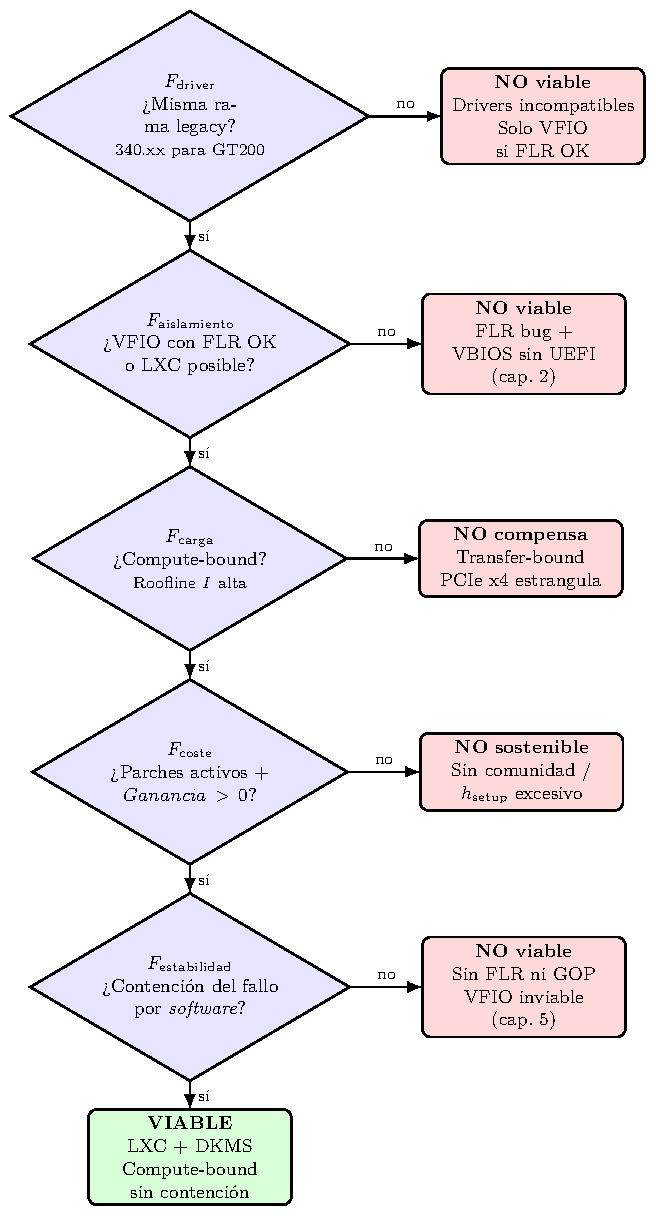
\includegraphics[height=0.60\textheight,keepaspectratio]{figuras/capitulo1/arbol-viabilidad}
\caption{\'Arbol de decisi\'on de viabilidad $V = F_{\text{driver}} \land F_{\text{aislamiento}} \land F_{\text{carga}} \land F_{\text{coste}} \land F_{\text{estabilidad}}$ aplicado al caso de estudio. Los cap\'itulos 2--5 recorren cada filtro en orden; $F_{\text{estabilidad}}$ se particulariza en la secci\'on~\ref{sec:marco_viabilidad} de los preliminares.}
\label{fig:arbol_viabilidad}
\end{figure}

\textbf{F1. Homogeneidad de driver} \cite{nvidia_legacy_driver,nvidia_legacy_support}. ¿Comparten todas las GPUs la misma rama legacy? En nuestro caso sí \cite{michelboucey}: GT200 $\to$ 340.108. Si no, la vía LXC queda bloqueada por la limitación del driver único descrita en este capítulo \cite{nvidia_forum_multidriver}; solo queda VFIO, que exige pasar al siguiente filtro.

\textbf{F2. Aislamiento} \cite{kernel_vfio,proxmox_pci_passthrough,supermicro_gpu_passthrough}. ¿La plataforma permite aislar cada GPU? Requiere IOMMU activa, grupo IOMMU dedicado \cite{heiko_iommu_groups} y FLR correcto \cite{pcisig2022,amd_pg344_flr}. Nuestro hardware falla en FLR (capítulo~2): VFIO inviable, pero LXC sí lo es porque comparte el driver del host y no necesita reset. Si ambos fallan, no hay vía.

\textbf{F3. Perfil de carga} \cite{williams2009roofline,amdahl1967}. ¿La aplicación es \textit{compute-bound}? Evaluar con Roofline: si $T_{\text{compute}} \gg B/BW_{\text{PCIe}}$ (ecuación de la sección~\ref{sec:roofline}), las lanes no importan. En el capítulo~\ref{cap5} demostramos que \texttt{matrixMul} lo es (sin contención con 2 GPUs concurrentes), por lo que el estrangulamiento PCIe del slot chipset no penaliza. Si la carga es \textit{transfer-bound}, la plataforma de consumo con x4 vía chipset \cite{asusx670e,amd7950x} hace que no compense frente a servidor con 64--128 lanes directas \cite{pcisig2022}.

\textbf{F4. Coste y sostenibilidad} \cite{michelboucey,archlinuxjerry}. ¿Existe mantenimiento comunitario y la ganancia supera el coste? Formalmente $Ganancia = S_{\text{real}}\cdot V_{\text{hora}} - (C_{\text{kWh}}\cdot h + C_{\text{ing}}\cdot h_{\text{setup}}) > 0$. El capítulo~3 cuantifica $h_{\text{setup}}$: 7 años de drift, 21 parches, toolchain gcc. Sin los repositorios comunitarios, $C_{\text{riesgo}}\to\infty$. Este es el filtro que convierte un éxito técnico puntual en un despliegue sostenible.

\textbf{F5. Estabilidad y contención del fallo} \cite{amd_pg344_flr,uefi_gop_amd}. ¿Existe algún mecanismo por \textit{software} capaz de recuperar una GPU colgada? Requiere, en el caso de VFIO, que el FLR funcione \cite{pcisig2022,amd_pg344_flr} y que la tarjeta disponga de GOP para el handover a la VM \cite{uefi_gop_amd}. En nuestro caso fallan ambos (capítulo~2), por lo que $F_{\text{estabilidad}}=\text{falso}$ y el despliegue se descarta como tal, tal y como se formaliza en la sección~\ref{sec:marco_viabilidad} de los preliminares.

La utilidad del marco es que anticipa el resultado sin necesidad de ejecutar: nuestro caso pasa F1--F4 pero falla F5 en la vía VFIO y solo se resuelve con LXC, que no requiere aislamiento; un caso con una Kepler (driver 470) + GT200 (340) fallaría ya en F1, y una carga de streaming fallaría en F3.


\chapter{Aislamiento de GPUs con máquinas virtuales} \label{cap2}

En este capítulo se aborda el segundo de los escenarios planteados en el capítulo 1: encapsular cada una de las tarjetas en una máquina virtual, cada una con su sistema operativo y su versión de driver correspondiente. Se describen los fundamentos del aislamiento de dispositivos, los obstáculos encontrados y el fallo documentado que llevó a descartar esta vía.

\section{Planteamiento}

Recordemos la situación de partida. Se disponía de tres GPUs NVIDIA que solo admiten la rama de driver 340.xx, aunque la configuración experimental empleó las dos tarjetas detectadas, y de
un sistema moderno (Proxmox VE) que difícilmente puede ejecutar esa rama sin parches. La idea de este capítulo 
es dar la vuelta al problema: en lugar de hacer que el host ejecute el driver antiguo, se crean máquinas virtuales 
con sistemas operativos con compatibilidad para ello, cada una de las cuales recibe una GPU en exclusiva mediante 
el paso directo de 
dispositivos (VFIO). Cada máquina virtual carga su propio driver, y la limitación del driver único queda superada 
por construcción.

Para que el \textit{passthrough} funcione, se necesita que el host cumpla tres condiciones \cite{proxmox_pci_passthrough,kernel_vfio,supermicro_gpu_passthrough}:

\begin{enumerate}
    \item Disponer de IOMMU activada, de forma que los accesos DMA de cada dispositivo queden restringidos a su espacio de direcciones virtual.

    \item Que la GPU objetivo constituya por sí sola un grupo IOMMU (o que todos los miembros del grupo puedan cederse), de modo que el kernel permita el aislamiento individual del dispositivo.

    \item Que el dispositivo soporte correctamente el \textbf{Function Level Reset}, de modo que al reiniciar la máquina virtual el 
    dispositivo pueda devolverse a un estado limpio y listo para el próximo arranque.
\end{enumerate}

\subsection{Ajustes de configuración específicos para VFIO}

Para el despliegue de esta fase experimental se diferenciaron dos niveles complementarios de virtualización asistida 
por hardware:

\begin{itemize}
    \item \textbf{SVM / AMD-V:} \textit{Secure Virtual Machine} (SVM) es el nombre de la arquitectura de instrucciones 
    que conforma la tecnología comercial AMD-V (\textit{AMD Virtualization}). Proporciona las extensiones de hardware 
    en el procesador necesarias para que el hipervisor KVM ejecute el código de las máquinas virtuales de forma nativa 
    en la CPU física.
    \item \textbf{AMD-Vi:} Constituye la implementación de AMD para la IOMMU 
    (\textit{I/O Memory Management Unit}), el circuito integrado encargado de traducir y restringir los 
    accesos directos a memoria física (\textit{Direct Memory Access}, DMA) emitidos por los periféricos.
\end{itemize}

En la configuración del firmware UEFI se habilitaron explícitamente ambas características: el modo SVM/AMD-V para permitir la
instanciación de máquinas virtuales completas, y AMD-Vi para que el \textit{kernel} de Linux estructurase los grupos IOMMU
necesarios para el aislamiento de cada GPU mediante el controlador \texttt{vfio-pci}.

Asimismo, fue necesario neutralizar \textit{Nouveau} ---el controlador libre y de código abierto 
para GPUs NVIDIA incluido por defecto en el núcleo de Linux---, ya que de lo contrario interferirá en 
la asignación de las tarjetas a \textit{vfio-pci}. Para impedirlo, 
se añadió el módulo a la lista negra (\textit{blacklist}) \cite{arch_nouveau}.

Los experimentos de este capítulo se ejecutaron seleccionando una sola vez la entrada VFIO del arranque dual descrito en el 
capítulo~\ref{cap1}; su uso operativo se resume en el apéndice~\ref{ape:manual-uso}.

\section{Evaluación experimental de passthrough mediante VFIO}

El objetivo de esta fase era comprobar si podíamos aislar cada una de nuestras tarjetas 
gráficas y pasárselas de forma exclusiva a una máquina virtual con KVM/QEMU vinculándolas
al módulo \texttt{vfio-pci}. 


\subsection{El primer tropiezo: la ASUS ENGTS250 no responde}

Tras arrancar el sistema con la configuración de VFIO mediante el script \texttt{boot-vfio}, 
comprobamos qué dispositivos se vinculan correctamente al controlador \texttt{vfio-pci}. 
Lo que cabía esperar era que al escanear el bus PCIe aparecieran las dos tarjetas conectadas: la Tesla C1060, en la
ranura principal, y la ASUS, en la ranura secundaria.
La sorpresa fue que en la lista únicamente figuraba la Tesla C1060; la ASUS ENGTS250 no aparecía.

Consultando los registros del \textit{kernel}, encontramos el origen del problema: 
un fallo durante la fase de negociación de la velocidad y anchura del bus PCIe (\textit{link training}). 
Este paso ocurre en la capa de enlace puramente física, mucho antes de que ningún controlador entre en juego. 
Al intentar aplicar un reinicio sobre la tarjeta, esta simplemente no contestó a tiempo, y el 
\textit{chipset} de la placa base la catalogó directamente como rota (\textit{broken device}) para no 
comprometer la estabilidad del resto del bus.

Este estado de bloqueo es crítico: una vez que el sistema coloca al dispositivo con esta marca, 
cesan todos los 
reintentos de comunicación. Ni siquiera conmutando entre configuraciones 
lograríamos devolver la tarjeta a su estado operativo. La tarjeta queda eléctricamente aislada, y un 
reinicio por software resulta inútil, por lo que hay que recurrir a un apagado manual completo (corte físico de 
corriente). Este debería ser siempre el último recurso, pues en un escenario sin acceso presencial al 
equipo dejaría el nodo totalmente inutilizable.

\subsection{Comprobaciones y ajustes en busca de una solución}

Antes de resignarnos con el peor escenario, se explora qué margen de 
maniobra exponen las tarjetas mediante software y configuración:

\paragraph{1. Inspección de los mecanismos de reinicio (Reset):}
Consultamos qué métodos de reinicio soportaba la tarjeta a través de \textit{sysfs}:
\begin{lstlisting}[language=bash]
$ cat /sys/bus/pci/devices/0000:08:00.0/reset_method
pm bus
\end{lstlisting}

Dado que la arquitectura de la familia GT200 carece de soporte por hardware para 
FLR (\textit{Function-Level Reset}), el \textit{kernel} debe recurrir a los mecanismos 
de contingencia expuestos por el dispositivo. La consulta a \texttt{reset\_method} confirmó 
que las únicas alternativas disponibles eran la transición de energía (\texttt{pm}) y el 
reinicio del bus, en este caso (\texttt{bus}, correspondiente al \textit{Secondary Bus Reset} o SBR) por estar
en la ranura compartida con el \textit{chipset}.

El método \texttt{pm} se apoya en el subsistema de gestión de energía PCI: fuerza al dispositivo 
a entrar en estado de bajo consumo \texttt{D3hot} (con alimentación presente pero relojes detenidos 
y pérdida del contexto interno) para devolverlo de inmediato a \texttt{D0} (rendimiento máximo), confiando en que la 
tarjeta se reinicie de forma limpia durante la transición \cite{kernel_pci_pm}. Sin embargo, 
en hardware de esta generación, dicha transición describe un comportamiento conocido, y por tanto,
mucho menos fiable. Ante esta incertidumbre, el \textit{kernel} 
se ve forzado a aplicar el método \texttt{bus} (SBR): una maniobra sustancialmente más agresiva que, 
al no poder aislar la GPU, induce una interrupción eléctrica abrupta sobre el 
enlace PCIe completo para forzar su reinicialización.

Este comportamiento resulta llamativo en lo relativo a las diferencias de comportamiento de las tarjetas durante las pruebas: 
a pesar de compartir una arquitectura muy similar, la inestabilidad y el colapso del bus se 
manifestaron de forma crítica en la ASUS ENGTS250 y no en la Tesla C1060. Como hipótesis de 
trabajo, la causa más plausible apunta a la topología física de conexión de cada tarjeta en 
la placa base. Mientras que la ranura principal de la Tesla se comunica a través de líneas 
PCIe dedicadas conectadas directamente a la CPU, la ASUS se encontraba instalada en una 
ranura secundaria subordinada a las líneas del \textit{chipset}. Al inducir un reinicio del bus secundario 
de bus (SBR) sobre un enlace intermediado por el \textit{chipset}, la perturbación eléctrica no 
solo afectó a la GPU, sino que desestabilizó el conmutador interno de dicho puente, arrastrando 
consigo a otros periféricos multiplexados en el mismo bus ---incluida la controladora de 
almacenamiento del \textit{host}--- y provocando el bloqueo total del sistema.

\paragraph{2. Control eléctrico del slot (Hotplug Power):}
Comprobamos si la placa base permite cortar la corriente de la ranura PCIe por software para 
emular el tirón de cable:
\begin{lstlisting}[language=bash]
$ ls /sys/bus/pci/slots/
\end{lstlisting}
El resultado fue negativo. La gestión de energía independiente por ranura es habitual en placas 
de servidor, pero inexistente en placas de consumo convencionales.

\paragraph{3. Desactivación de mecanismos de ahorro de energía:}
La hipótesis de trabajo era que las funciones de gestión de energía del PCIe estaban 
mandando a la tarjeta a estados de reposo de los que luego era incapaz de despertar a tiempo. 
Por ello, aplicamos una serie de directivas agresivas en la línea de comandos del \textit{kernel} 
(\texttt{cmdline}) y en la BIOS:
\begin{itemize}
    \item \textbf{\texttt{vfio\_pci.disable\_idle\_d3=1}:} Evita que el controlador ponga la GPU en 
    reposo profundo ($D3_{hot}$) mientras la máquina virtual no la usa. Al ser la tarjeta tan antigua, 
    los comportamientos no son predecibles.
    \item \textbf{\texttt{pcie\_aspm=off}:} Deshabilita por completo el ahorro de energía en el propio 
    enlace físico PCIe (\textit{Active-State Power Management}).
    \item \textbf{\texttt{pcie\_port\_pm=off}:} Desactiva la gestión de energía en el puente 
    PCIe que da acceso a la GTS250. Este parámetro fue determinante para evitar que el puente del que cuelga la GPU
    cortase la comunicación durante la reconfiguración.
    \item \textbf{\texttt{pci=noaer}:} Desactiva el reporte avanzado de errores para evitar que el 
    sistema sobrerreaccione ante pequeñas inestabilidades del enlace. Este parámetro más que solucionar un problema
    en caso de haberlo, lo enmascararía.
\end{itemize}

Tras forzar la modificación de estos parámetros, se consiguió que ambas GPUs, Tesla C1060 y ahora también la ASUS ENGTS 250,
se vinculasen al módulo \textit{vfio}.
De entre los parámetros modificados, la principal sospecha de éxito recayó en \texttt{vfio\_pci.disable\_idle\_d3=1}: 
impedir que VFIO dejara la GPU en \texttt{D3hot} eliminaba una transición energética problemática. 
No obstante, como todas estas directivas se aplicaron conjuntamente, su efecto 
individual no quedó aislado; esta explicación es coherente con el momento del cuelgue, pero no demuestra por sí 
sola cuál fue el parámetro determinante. Sabiendo que con estas pruebas estábamos exponiendo al sistema a comportamientos
eléctricos no conocidos, se decidió dar por válida la vinculación sin determinar cuál de los parámetros exactos 
nos hizo avanzar.


Así pues con estos cambios conseguimos el primer gran avance: la ASUS ENGTS250 completó el \textit{binding} 
con \texttt{vfio-pci} de forma consistente. La negociación se estabilizó a menor velocidad ($\times 4$ 
a 2.5 GT/s en lugar de sus $\times 16$ nominales), lo que ralentizaba ligeramente el arranque, pero 
al menos habíamos eliminado el cuelgue eléctrico inicial.

\subsection{La prueba de fuego en la máquina virtual y el cuelgue definitivo}

Con el controlador \texttt{vfio-pci} adueñado de la tarjeta, lo siguiente era comprobar si podíamos levantar 
una máquina virtual funcional. Diseñamos un protocolo de validación adaptado a las limitaciones 
heredadas de las tarjetas:
\begin{enumerate}
    \item Se configuró la máquina virtual con \textbf{SeaBIOS} (emulación de BIOS clásica de 16 bits) 
    y tipo de máquina \textbf{i440fx}, debido a la ausencia de GOP en la VBIOS de la GPU.
    \item Se instaló el sistema operativo base sin la GPU conectada para evitar interferencias.
    \item Se añadió la tarjeta gráfica mediante la directiva \texttt{hostpci0: 08:00.0}, aplicando dos 
    precauciones clave:
    \begin{itemize}
        \item \textbf{Desactivar la lectura de la ROM (\texttt{rombar=0}):} Evita que QEMU exponga 
        la memoria ROM de la tarjeta (\textit{Expansion ROM BAR}) a la máquina virtual. En tarjetas 
        antiguas, el acceso y mapeo de esta región de memoria entra en conflicto con los registros 
        de control principales (BAR0/MMIO) del dispositivo una vez que este ya ha sido inicializado. 
        Dado que la GPU se destina exclusivamente a tareas de cómputo y no a la salida gráfica del 
        arranque de la VM, la exposición de la VBIOS resulta innecesaria y su desactivación elimina 
        bloqueos por contención en el bus.
        \item \textbf{Desactivación de la GPU primaria (\texttt{x-vga=0}):} Evita que el hipervisor 
        trate a la GPU física como el adaptador VGA principal de la máquina virtual. 
        En su lugar, se configuró una tarjeta gráfica virtual emulada 
        (\textit{VirtIO-GPU}), la cual redirige la salida de vídeo del sistema operativo invitado hacia 
        la consola web del hipervisor mediante el protocolo noVNC (cliente VNC integrado en la interfaz 
        de Proxmox). De este modo, la GTS250 queda liberada de cualquier función de salida de vídeo, 
        quedando asignada como acelerador secundario dedicado exclusivamente a cómputo.
    \end{itemize}
\end{enumerate}

Pese a todas las precauciones, en el momento exacto en que la máquina virtual intentó arrancar e 
inicializar la tarjeta, el sistema anfitrión se congeló por completo, obligando de nuevo a forzar el 
apagado manual del equipo. 

Como detalle relevante, la interfaz de Proxmox reportó la máquina virtual como iniciada con éxito
mientras el equipo ya estaba totalmente bloqueado; un claro falso positivo en la monitorización. 
Esta prueba confirmó de manera empírica que, aun resolviendo los problemas del enlace físico a base de 
parámetros en el \textit{kernel}, la incapacidad de estas tarjetas antiguas para recuperarse de un reinicio por 
software hace inviable su uso estable mediante VFIO en nuestra plataforma.

\section{Resultado y decisión}

Tras múltiples intentos de configuración (activación de IOMMU en la BIOS, reserva de las GPUs con el módulo \texttt{vfio-pci}, pases de ID de dispositivo, etc.), el despliegue de las VMs con VFIO se descartó por inviable:

\begin{itemize}
    \item La ausencia de \textbf{FLR} de ambas tarjetas impide la reutilización del dispositivo
entre máquinas virtuales: el ciclo de vida de la VM (apagado $\rightarrow$ reinicio) deja la GPU
inaccesible eléctricamente.
\end{itemize}

Como se mencionó anteriormente, por integridad del sistema, 
se decidió no repetir sistemáticamente estos bloqueos eléctricos: cada cuelgue exigía un apagado manual y 
exponía el sistema de ficheros y el arranque a nuevos daños. La conclusión se apoya, por tanto, en la repetición 
del patrón de fallo y en su coherencia con la ausencia de recuperación por software, ya que el apagado manual
no es ni solución definitiva ni robusta.

\section{Análisis comparativo: máquinas virtuales frente a contenedores}

A la vista de lo experimentado en este capítulo, la tabla \ref{tab:vm-lxc} resume la comparación 
cualitativa entre las dos vías de compartición de GPUs analizadas hasta ahora. Aunque el capítulo 3 y 
siguientes desarrollan la vía de los contenedores, anticipar aquí la comparación ayuda a situar el fallo 
de este capítulo en su contexto: no se trata de una vía desaconsejada en términos generales, sino de una vía inadecuada para 
las características concretas de nuestro hardware.

\begin{table}[htbp]
\centering
\singlespacing
\footnotesize
\setlength{\tabcolsep}{4pt}
\begin{tabularx}{\textwidth}{|>{\raggedright\arraybackslash}p{2.7cm}|>{\raggedright\arraybackslash}X|>{\raggedright\arraybackslash}X|}
\hline
\textbf{Criterio} & \textbf{Máquina virtual (VFIO)} & \textbf{Contenedor LXC} \\
\hline
Aislamiento del hardware & Total (dispositivo dedicado) & Compartido (\textit{device nodes} del host) \\
\hline
Versiones de driver & Una distinta por VM & Una única para todo el sistema \\
\hline
Requisitos de plataforma & IOMMU activa, grupos IOMMU, FLR correcto & Ninguno \\
\hline
Reinicio del dispositivo & Necesita reset limpio (FLR); crítico para el ciclo de vida de la VM & No interviene: el driver sigue en el host \\
\hline
Coste de configuración & Alto (BIOS, \texttt{vfio-pci}, ROM de vídeo) & Bajo (\textit{cgroup} + \textit{bind mount}) \\
\hline
Uso conjunto con el host & Imposible (GPU exclusiva de la VM) & Posible (driver compartido) \\
\hline
Idoneidad con hardware \textit{legacy} & Mala (FLR incompleto, VBIOS sin UEFI) & Buena (el driver lo resuelve el host) \\
\hline
\end{tabularx}
\caption{Comparación cualitativa entre máquinas virtuales y contenedores para la compartición de GPUs}
\label{tab:vm-lxc}
\end{table}

La conclusión de este capítulo es que la virtualización completa no es la vía adecuada para integrar GPUs 
\textit{legacy} en sistemas modernos. No obstante, el análisis no fue en vano: delimitó con precisión 
las condiciones que debe cumplir cualquier vía alternativa. La vía de los contenedores LXC, que se estudia en 
el capítulo siguiente, no necesita ni IOMMU ni reset de dispositivos, ya que el contenedor comparte el kernel 
del host y, por tanto, el propio driver que ya controla las tarjetas. La contrapartida es volver a la limitación 
del driver único: solo puede haber un driver propietario en el sistema. 


\chapter{Pivote a LXC: el driver legacy en Proxmox VE} \label{cap3}

\section{Por qué LXC}

La tecnología de contenedores LXC presenta, frente a las máquinas virtuales, una diferencia fundamental:
 los contenedores comparten el kernel del host. Esta característica, que en el capítulo 2 nos parecía 
 una limitación, es precisamente la clave de esta fase. Al compartir el kernel, el contenedor no 
 necesita un driver propio: usa el módulo del driver NVIDIA que carga el host, y solo necesita montar
 los \textit{character devices} correspondientes. No hay IOMMU, no hay grupos, no hay 
 resets: el aislamiento a nivel de hardware no interviene.

La contrapartida es inmediata: volvemos a la limitación del driver único. Solo puede haber un driver
propietario de NVIDIA a nivel de sistema, y ese driver debe ser capaz de controlar todas las GPUs. 
Como hasta ahora ambas tarjetas de pruebas comparten la misma rama \textit{legacy} (340.xx), 
consideramos que valía la pena hacer la prueba. El problema se traslada entonces de la virtualización a 
la instalación del driver: conseguir que el driver 340.108 ---con el último \textit{release} oficial en 2019--- 
funcione sobre un kernel de 2026.

\section{Diagnóstico de la incompatibilidad fundamental} \label{sec:cap3-diagnostico}

Para entender el origen de la incompatibilidad conviene recordar cómo se integra un driver en Linux. Un driver como el de NVIDIA no es un programa independiente, sino un \textit{módulo} que se carga dentro del propio kernel. Para construirlo hay que compilar su código fuente contra los \textit{headers} del kernel ---los ficheros que describen la estructura interna del mismo--- y con un compilador (gcc) compatible con el que se usó para compilar ese kernel. Si alguna de estas tres piezas (código del driver, \textit{headers} y compilador) no encaja con las demás, el módulo no puede compilarse. Además, como el módulo resultante queda ligado a la versión concreta del kernel para la que se compiló, debe recompilarse cada vez que el kernel se actualiza. De esta tarea se encarga habitualmente DKMS (\textit{Dynamic Kernel Module Support}), una herramienta que recompila de forma automática los módulos externos al kernel tras cada actualización.

El driver NVIDIA 340.108 fue diseñado contra kernels de la serie 3.x/4.x. El kernel por defecto de Proxmox VE 9.2 
(serie 6.x/7.x, de 2025--2026) presenta una diferencia de aproximadamente siete años de evolución de la API 
interna del kernel (gestión de memoria, macros de compilación, etc.). No es de extrañar que el código fuente del driver no 
compile sin más 
contra los \textit{headers} modernos.

Esta distancia temporal es especialmente problemática en Linux: las distintas versiones del kernel no mantienen un patrón 
estable en la 
interfaz interna para los módulos, ni a nivel de código fuente (API) ni a nivel binario (ABI). Cuando 
esta interfaz cambia, los drivers incluidos en el propio kernel se adaptan a la vez, pero un driver externo como el de 
NVIDIA depende de que su fabricante ---o, en su defecto, la comunidad--- lo actualice. Sin esa actualización, cuanto 
mayor es la distancia entre versiones, más llamadas del driver dejan de existir o cambian de firma, lo que explica la 
gran cantidad de errores de compilación que se describen más adelante.

Una comparación con el capítulo 1 ayuda a situar el problema: en Ubuntu 18.04 (kernel 4.15, gcc 7.x, apenas dos años 
de diferencia respecto al driver), el paquete \texttt{nvidia-340} instalaba sin complicaciones porque se mantienen 
binarios y parches adaptados para ello de forma oficial. Para combinaciones de kernel tan recientes como las de este trabajo, 
\textbf{ningún repositorio oficial mantiene el driver 340.xx}: la tabla de plazos de soporte de NVIDIA 
declara expresamente que la serie 340.* es la última que da soporte a las GPUs G8x, G9x y GT2xx, que la 
compatibilidad con kernels Linux se cerró en la versión 340.108 y que no está prevista ninguna publicación
posterior de la serie \cite{nvidia_legacy_support,nvidia_legacy_gpu}. Por tanto, la compilación debe abordarse 
manualmente o mediante parches de terceros mantenidos por la comunidad, si es que existen.

\section{Bitácora de resolución de problemas}

A continuación se resumen, siguiendo a grandes rasgos el orden en que se presentaron, los obstáculos encontrados hasta conseguir que el driver funcionase. El objetivo no es reproducir cada orden ejecutada, sino explicar qué falló, por qué, y qué enseña cada problema sobre la viabilidad de este tipo de sistemas. Los pasos para reproducir la instalación se resumen en el apéndice~\ref{ape:host}, y la relación completa de problemas y causas raíz, en el apéndice~\ref{ape:causas-raiz}.

No todos los obstáculos tuvieron el mismo peso. La mayoría fueron incidencias menores de configuración, resueltas con rapidez, mientras que uno de ellos ---el fallo estructural de la compilación manual--- obligó a cambiar por completo de estrategia.

\subsection{Preparación del host y del entorno de compilación} \label{sec:cap3-preparacion}

El primer paso fue liberar las GPUs de la configuración heredada del capítulo~\ref{cap2}. Durante los 
experimentos con VFIO, las tarjetas habían quedado reservadas desde el arranque para \texttt{vfio-pci}, 
el módulo que las aparta del host para cedérselas a una máquina virtual, de modo que ningún driver del host 
podía tomar su control. Este paso puso de manifiesto que ambos enfoques son incompatibles por naturaleza: 
VFIO necesita reservar el hardware del host, mientras que LXC necesita que el host lo gobierne. Por ello, 
además de revertir la configuración para aislamiento, se diseñó el sistema de arranque dual descrito en la sección~\ref{sec:arranque},
que permite alternar limpiamente entre ambas configuraciones en cada inicio.

A continuación se abordó la elección del kernel. El que Proxmox VE 9.2 instala por defecto (versión 7.0) era demasiado moderno para el driver, por lo que se instaló y fijó como kernel de arranque una versión anterior también soportada por Proxmox, la 6.14. Este cambio, sin embargo,
no fue suficiente: incluso con la versión 6.14 seguía sin haber paquetes precompilados ni parches oficiales, y la diferencia entre driver y kernel seguía siendo demasiado grande para compilar el driver sin modificar su código.

Durante esta preparación surgieron además dos incidencias menores. Por un lado, el instalador no encontraba los \textit{headers} del kernel porque Proxmox VE 9 había cambiado el nombre del paquete que los contiene (de \texttt{pve-headers} a \texttt{proxmox-headers}), un ejemplo de cómo buena parte de la documentación disponible para software antiguo ha quedado desactualizada. Por otro, el instalador de NVIDIA detenía la instalación al detectar que el kernel se había compilado con gcc 12.2 y el sistema disponía de gcc 12.4. Aunque se trata de una diferencia menor que el propio kernel solo trata como un aviso, fue necesario indicar expresamente al driver que ignorase esta comprobación, tanto en el instalador como, más adelante, en la configuración de DKMS.

\subsection{Intentos de compilación manual sin parches} \label{sec:cap3-manual}

Con los requisitos previos resueltos, se intentó compilar el driver manualmente y sin modificar su código, aun
sabiendo que era un camino costoso en complejidad y en tiempo. Algunos de los errores pudieron resolverse
ajustando directivas de compilación, pero, como se verá, resolverlos todos de esta forma no era viable
ni habría dado lugar a una solución robusta.

Los primeros errores fueron de configuración del entorno: la convivencia de varias versiones de gcc y la modificación manual de las opciones de compilación impedían localizar algunos ficheros, tanto del compilador como del propio driver, y se resolvieron con ajustes puntuales. El siguiente, en cambio, fue estructural: incluso con los anteriores resueltos, la compilación terminó en cientos de errores encadenados como los siguientes:
\begin{lstlisting}[style=bash]
error: unknown type name 'nv_state_t'
error: request for member 'flags' in something not a structure or union
\end{lstlisting}

Su origen está en el mecanismo con el que el driver se adapta a cada kernel. Como el kernel cambia de una versión a otra, el driver incluye un script llamado \texttt{conftest} que, antes de compilar, realiza pequeñas pruebas sobre los \textit{headers} del kernel de destino para averiguar qué estructuras y funciones ofrece y qué versión de gcc emplea, y con ello genera un fichero de configuración (\texttt{conftest.h}) con las definiciones que necesita el resto del código. Al haber modificado manualmente las opciones de compilación, este mecanismo no llegó a ejecutarse correctamente, y el driver se compiló sin información sobre la configuración del kernel de destino. El error se repitió en todos los intentos de compilación manual.

Este fallo marcó el final de la vía manual. Con tanta distancia entre versiones, no basta con ajustar la compilación: el propio código del driver debe modificarse para adaptarse a los cambios internos del kernel. Por ello se recurrió a un conjunto de parches ya mantenido por la comunidad.

\section{Los parches comunitarios y la solución con DKMS}

Si en Ubuntu 18.04 el mismo driver se instalaba sin dificultad (capítulo~\ref{cap1}), es porque la propia 
distribución mantenía parches para adaptarlo a su kernel. Para un kernel actual, ese trabajo lo realizan 
repositorios mantenidos por la comunidad. 

\subsection{De la compilación manual a DKMS} \label{sec:cap3-parches}

La incorporación de los parches comunitarios se realizó en dos intentos, que se diferencian en dos aspectos: el repositorio de parches empleado y la forma de compilar el driver. Distinguir ambos aspectos es clave para entender por qué el primero fracasó y el segundo no.

En el primer intento se utilizó el repositorio \texttt{dkosmari/nvidia-340.108-updated} \cite{dkosmari}, que reúne todas las modificaciones en un único parche. El parche se aplicó sin problemas sobre el código original del driver \cite{nvidia_340_driver_file}, de modo que el código ya quedaba adaptado al kernel moderno. Sin embargo, la compilación se siguió realizando igual que en la sección~\ref{sec:cap3-manual}: invocando directamente la orden de compilación con opciones ajustadas manualmente. Como consecuencia, el mecanismo \texttt{conftest} volvió a no ejecutarse correctamente y la compilación falló por el mismo motivo. Este intento demostró que parchear el código era necesario, pero no suficiente: también había que cambiar la forma de compilarlo.

En el segundo intento se cambiaron ambos aspectos. Por un lado, la compilación se delegó en DKMS. Además de recompilar el módulo tras cada actualización del kernel, DKMS ejecuta el proceso de compilación tal y como lo define el propio driver en su fichero de configuración (\texttt{dkms.conf}), sin intervenir manualmente en las opciones de compilación. De este modo, el mecanismo \texttt{conftest} se ejecuta como el driver espera, lo cual era precisamente lo que había fallado en todos los intentos anteriores. Por otro lado, se sustituyó el parche único por el repositorio \texttt{MichelBoucey/nvidia-340xx} \cite{michelboucey}, derivado de \texttt{archlinux-jerry/nvidia-340xx} \cite{archlinuxjerry} y mantenido activamente. Frente a un parche único y genérico, este repositorio ofrece parches específicos para versiones concretas del kernel, entre ellas la 6.14 empleada en este trabajo, lo que ofrecía mayores garantías de compatibilidad con el entorno. Por ese motivo, no se llegó a probar el primer repositorio con DKMS. Además, el nuevo repositorio está preparado para integrarse con DKMS: uno de sus parches deja lista la configuración que este necesita, a la que solo hubo que añadir la indicación de ignorar la comprobación de versión del compilador descrita en la sección~\ref{sec:cap3-preparacion}.

Estos parches son incrementales y adaptan el driver a las sucesivas versiones del kernel (de la 5.7 a la 7.0) y del compilador (gcc 14 y 15). Como el kernel se había fijado en la versión 6.14, solo correspondía aplicar los parches necesarios hasta esa versión; los destinados a kernels posteriores, también incluidos en el repositorio, no eran necesarios. Los 21 parches aplicados se integraron sin ningún fallo.

La tabla~\ref{tab:intentos-compilacion} resume la evolución de los intentos de compilación descritos hasta aquí.

\begin{table}[htbp]
\centering
\small
\setlength{\tabcolsep}{4pt}
\begin{tabular}{|L{3.4cm}|L{3.0cm}|L{2.6cm}|L{4.2cm}|}
\hline
\textbf{Intento} & \textbf{Código del driver} & \textbf{Compilación} & \textbf{Resultado} \\
\hline
Sin parches (sección~\ref{sec:cap3-manual}) & Original & Manual & Falla: código no adaptado y \texttt{conftest} sin ejecutar \\
\hline
Repositorio \texttt{dkosmari} & Parche único & Manual & Falla: \texttt{conftest} sin ejecutar \\
\hline
Repositorio \texttt{MichelBoucey} & Parches incrementales & DKMS & Éxito, tras corregir una opción de compilación \\
\hline
\end{tabular}
\caption{Evolución de los intentos de compilación del driver}
\label{tab:intentos-compilacion}
\end{table}

Gracias a DKMS, el módulo se recompilará automáticamente con cada actualización del kernel, en lugar de quedar como un binario congelado, válido solo para la versión actual, que habría que recompilar manualmente.

Por último, se instalaron los componentes del driver que no forman parte del kernel (librerías y herramientas como \texttt{nvidia-smi}), indicando al instalador oficial que no volviera a compilar el módulo. Se descartaron las librerías de 32 bits y la configuración del entorno gráfico, innecesarias en un servidor sin interfaz gráfica.

\section{Verificación y consideraciones sobre el módulo UVM}

Ejecutamos \texttt{nvidia-smi} y comprobamos que el driver detecta ambas GPUs sin problemas. La instalación quedó además verificada tras un ciclo completo de arranque, confirmando la persistencia del módulo vía DKMS.

Un aspecto técnico relevante de esta fase es la decisión deliberada de no compilar el segundo módulo que suele acompañar al driver, \texttt{nvidia-uvm.ko}. Como se explicó en los preliminares, UVM (\textit{Unified Virtual Memory}) es un sistema de memoria virtual unificada compartido entre CPU y GPU \cite{nvidia_uvm_docs}. Sin UVM, la RAM y la VRAM son dos espacios completamente aislados: el programador debe reservar memoria por separado en cada uno de ellos y copiar explícitamente los datos de la CPU a la GPU y de vuelta. Con UVM, ambos espacios se perciben como uno solo, y basta con una única reserva. El intercambio de datos se resuelve mediante \textit{page faulting} por hardware, de forma muy similar a la paginación de los sistemas operativos: cuando se accede a una dirección que no está cargada, el módulo \texttt{uvm} intercepta el fallo y trae la página correspondiente, consultando unas tablas que indican dónde se encuentra cada una (CPU, GPU o ambas).

Las GPUs de las que disponemos son previas a la introducción de UVM en el hardware, por lo que todas las limitaciones descritas 
nos afectan de forma directa,
al no estar soportada la memoria unificada en estas tarjetas.
La decisión de no compilar el módulo \texttt{nvidia-uvm.ko} se validó empíricamente en el capítulo 5, cuando \texttt{deviceQuery} confirmó que ambas tarjetas reportan \texttt{Device supports Unified Addressing (UVA): No}.

\section{Discusión}

La tabla \ref{tab:causas-resumen} resume los obstáculos de esta fase agrupados por categoría, de modo que pueda apreciarse la naturaleza del problema en conjunto; la versión completa, problema a problema, se recoge en el apéndice~\ref{ape:causas-raiz}.

\begin{table}[H]
\centering
\small
\setlength{\tabcolsep}{4pt}
\begin{tabular}{|L{4.0cm}|L{7.8cm}|}
\hline
\textbf{Categoría} & \textbf{Problemas agrupados} \\
\hline
Configuración del host & Residuos de la configuración VFIO previa (1 problema) \\
\hline
Empaquetado / documentación & Cambio de nomenclatura \texttt{pve-*} $\rightarrow$ \texttt{proxmox-*}; plantilla de contenedor con \textit{build} cambiante (2) \\
\hline
Obsolescencia del software \textit{legacy} & Driver de 2019 frente a kernel de 2026; front-end de \texttt{nvcc} 6.5 frente a cabeceras C++11; instaladores rotos de CUDA (4) \\
\hline
Configuración de \textit{toolchain} & Múltiples gcc coexistentes, \texttt{-nostdinc}, checks estrictos del instalador (3) \\
\hline
Metodología de compilación & Fallo de \texttt{conftest} al sobrescribir flags manualmente; necesidad de extracción manual por capas (3) \\
\hline
Mantenimiento de terceros & Dependencia de parches comunitarios para la compatibilidad del driver (2) \\
\hline
\end{tabular}
\caption{Causas raíz de la fase de instalación del driver, agrupadas por categoría}
\label{tab:causas-resumen}
\end{table}

El resultado más relevante de este capítulo es que la viabilidad de ejecutar hardware NVIDIA de la arquitectura Tesla (2008--2009) en un host con kernel y \textit{toolchain} de 2025--2026 \textbf{depende enteramente de la existencia y mantenimiento activo de parches de terceros}, dado que NVIDIA no ofrece soporte oficial para esta combinación desde hace varios años. La reproducibilidad del proceso está, por tanto, sujeta a la disponibilidad continuada de dichos parches, un riesgo que debe tenerse en cuenta al valorar este tipo de despliegues.

Desde el punto de vista metodológico, el proceso confirma la importancia de utilizar \textit{toolchains} gestionados (DKMS) frente a invocaciones manuales de \texttt{make}, y la conveniencia de fijar versiones de compilador mediante \texttt{update-alternatives} para evitar interacciones entre múltiples versiones de gcc. En términos cualitativos, la conclusión general de la fase es doble: el \textbf{obstáculo dominante} no es el hardware (que funciona correctamente bajo el driver correcto), sino la \textbf{obsolescencia del software}, y el \textbf{factor habilitante} es la existencia de una comunidad que mantiene vivo el soporte de estos drivers. Sin esa comunidad, el aprovechamiento de estas tarjetas sería directamente inviable, lo que sitúa el mantenimiento comunitario como un criterio de viabilidad de primer orden en la evaluación de sistemas con hardware \textit{legacy}. El procedimiento completo y reproducible, sin la traza de errores, se recoge en el apéndice~\ref{ape:host}.

Con el driver funcionando en el host y ambas GPUs detectadas, el siguiente paso, que se aborda en el capítulo 4, es proporcionar acceso a las tarjetas a un contenedor LXC e instalar el stack de cómputo CUDA compatible.


\chapter{Contenedor LXC con acceso a GPU y stack CUDA 6.5} \label{cap4}

En este capítulo se describe la configuración del contenedor LXC con acceso directo a ambas GPUs, la instalación del stack \textit{userspace} de NVIDIA dentro del contenedor y la instalación del último toolkit CUDA compatible con las arquitecturas del hardware (CUDA 6.5). El capítulo culmina con la validación del cómputo real mediante \texttt{deviceQuery}.

\section{Objetivo}

Partimos de la situación alcanzada en el capítulo 3: el driver 340.108 está instalado y funcionando en el host vía DKMS, con \texttt{nvidia-smi} operativo y detectando ambas tarjetas. El objetivo ahora es crear un contenedor LXC en Proxmox VE 9 con acceso directo (paso de dispositivos) a ambas GPUs, e instalar dentro de él el stack CUDA 6.5 para validar cómputo real.

La figura \ref{fig:arquitectura} resume la arquitectura del sistema completo en su estado final: el host Proxmox carga el módulo de kernel del driver (único driver del sistema), y el contenedor \texttt{gpu-tfg} accede a las tarjetas mediante \textit{bind mounts} de los \textit{character devices}.

\begin{figure}[htbp]
\centering
% Figura precompilada para reducir el tiempo de compilacion.
% Fuente editable: figuras/capitulo4/arquitectura-sistema.tex
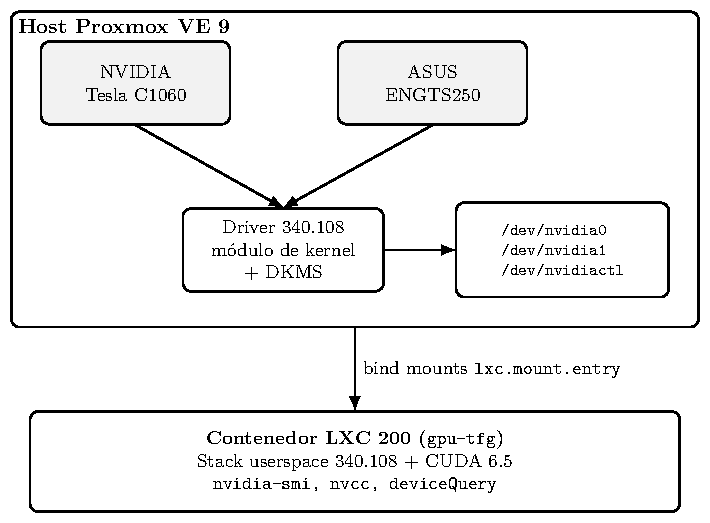
\includegraphics{figuras/capitulo4/arquitectura-sistema}
\caption{Arquitectura del sistema: host Proxmox con el driver, y contenedor LXC con acceso a ambas GPUs}
\label{fig:arquitectura}
\end{figure}

\section{Selección de almacenamiento}

Antes de crear el contenedor se verificó el almacenamiento disponible en Proxmox con \texttt{pvesm status}, que arrojó dos \textit{storages} con usos complementarios (tabla \ref{tab:storage}):

\begin{table}[htbp]
\centering
\begin{tabular}{|l|l|l|}
\hline
\textbf{Storage} & \textbf{Tipo} & \textbf{Uso recomendado} \\
\hline
\texttt{local} & \texttt{dir} & Plantillas (\texttt{vztmpl}), ISOs, backups \\
\hline
\texttt{local-lvm} & \texttt{lvmthin} & Discos de VMs y rootfs de contenedores \\
\hline
\end{tabular}
\caption{Almacenamiento disponible en Proxmox}
\label{tab:storage}
\end{table}

Se decidió usar \texttt{local-lvm} para el \textit{rootfs} del contenedor y \texttt{local} únicamente como origen de la plantilla de sistema.

\section{Obtención de la plantilla de sistema}

La plantilla se obtiene con \texttt{pveam} (administrador de plantillas de contenedores): \texttt{pveam update}, \texttt{pveam available} y \texttt{pveam download}. Una observación importante de esta fase es que el nombre exacto de la plantilla (número de \textit{build} tras \texttt{debian-12-standard\_12.X-1\_amd64.tar.zst}) varía con el tiempo según lo que Proxmox tenga indexado en el momento; debe consultarse siempre con \texttt{pveam available} antes de descargar, en lugar de asumir una versión fija.

\section{Creación del contenedor}

El contenedor se creó con el siguiente comando:

\begin{lstlisting}[style=bash]
pct create 200 local:vztmpl/<plantilla>.tar.zst \
  --hostname gpu-tfg \
  --cores 4 \
  --memory 4096 \
  --rootfs local-lvm:32 \
  --net0 name=eth0,bridge=vmbr0,ip=dhcp \
  --unprivileged 0 \
  --features nesting=1
\end{lstlisting}

Dos decisiones de diseño son relevantes. En primer lugar, se optó deliberadamente por un \textbf{contenedor privilegiado} en lugar de no privilegiado. Los contenedores no privilegiados aplican un remapeo de UID/GID entre el \textit{namespace} del contenedor y el host \cite{lxc_security,lxc_containers_conf}, lo que complica significativamente el acceso a \textit{character devices} como los de NVIDIA (habría que mapear también los grupos propietarios de \texttt{/dev/nvidia*}). Para un entorno experimental como el de este trabajo, la vía privilegiada es la más simple y directa, a costa de un aislamiento de seguridad menor, una decisión razonable dado el contexto puramente experimental del proyecto.

En segundo lugar, \texttt{--features nesting=1} prepara el contenedor por si se requiere anidar otros entornos (Docker, otro LXC) en fases posteriores.

\section{Identificación de los device nodes en el host}

El siguiente paso es identificar los \textit{device nodes} que expone el driver en el host. El resultado relevante de \texttt{cat /proc/devices | grep -i nvidia} es:

\begin{lstlisting}[style=bash]
195 nvidia-frontend
\end{lstlisting}

El \textit{major} 195 corresponde al \textit{frontend} del driver NVIDIA y es el que expone \texttt{/dev/nvidia0}, \texttt{/dev/nvidia1} y \texttt{/dev/nvidiactl}. No aparece ningún \textit{major} para \texttt{nvidia-uvm} porque el módulo \texttt{nvidia-uvm.ko} no se compiló deliberadamente (véase el capítulo 3); por tanto, la configuración del contenedor no incluye el bloque de paso de dispositivo para UVM.

El mapeo de GPUs, confirmado con \texttt{nvidia-smi} en el host, es:

\begin{table}[htbp]
\centering
\begin{tabular}{|l|l|l|}
\hline
\textbf{Device node} & \textbf{GPU} & \textbf{Bus PCI} \\
\hline
\texttt{/dev/nvidia0} & Tesla C1060 & \texttt{0000:01:00.0} \\
\hline
\texttt{/dev/nvidia1} & GeForce GTS 250 (ENGTS250) & \texttt{0000:08:00.0} \\
\hline
\texttt{/dev/nvidiactl} & (control, compartido) & --- \\
\hline
\end{tabular}
\caption{Mapeo de device nodes a GPUs en el host}
\label{tab:devices}
\end{table}

\section{Configuración del paso de dispositivos}

La configuración del contenedor se realiza en \texttt{/etc/pve/lxc/200.conf}, añadiendo el permiso de \textit{cgroup} sobre el \textit{major} del driver y los \textit{bind mounts} de cada dispositivo:

\begin{lstlisting}[style=bash]
lxc.cgroup2.devices.allow: c 195:* rwm
lxc.mount.entry: /dev/nvidia0 dev/nvidia0 none bind,optional,create=file
lxc.mount.entry: /dev/nvidia1 dev/nvidia1 none bind,optional,create=file
lxc.mount.entry: /dev/nvidiactl dev/nvidiactl none bind,optional,create=file
\end{lstlisting}

Esta configuración proporciona acceso a \textbf{ambas GPUs simultáneamente} desde el mismo contenedor. Para un escenario de aislamiento por GPU (un contenedor por tarjeta, de interés para comparativas de rendimiento aisladas), bastaría con omitir el \texttt{lxc.mount.entry} de la GPU no deseada en cada \texttt{.conf} respectivo.

Antes de arrancar el contenedor es necesario comprobar que los nodos existen en el host; si no, se fuerza su creación ejecutando \texttt{nvidia-smi} una vez. Tras el arranque (\texttt{pct start 200}), se confirmó que los tres \textit{device nodes} (\texttt{nvidia0}, \texttt{nvidia1}, \texttt{nvidiactl}) llegan correctamente al \textit{namespace} del contenedor con el mismo \textit{major} 195.

\section{Instalación del stack userspace NVIDIA en el contenedor}

A diferencia del módulo de kernel, que requirió el proceso extenso de parcheo documentado en el capítulo 3, el stack \textit{userspace} (librerías \texttt{libcuda}, \texttt{nvidia-smi}, etc.) es un binario precompilado por NVIDIA y \textbf{no depende de dichos parches}. Por tanto, dentro del contenedor se utiliza el instalador \texttt{.run} oficial sin modificar, únicamente con el flag \texttt{--no-kernel-module} que omite la instalación del módulo de kernel (compartido con el host). Los \textit{prompts} respondidos durante la instalación son idénticos a los del host y por el mismo motivo (entorno sin X11): no instalar las librerías de compatibilidad de 32 bits y no generar configuración X11.

La verificación con \texttt{nvidia-smi} confirma que ambas GPUs son visibles y accesibles desde dentro del contenedor, con la misma versión de driver (340.108) que el host, validando la compatibilidad ABI entre el módulo de kernel (host) y las librerías \textit{userspace} (contenedor).

\section{CUDA Toolkit 6.5}

\subsection{Justificación de la versión}

Las \textit{compute capabilities} de las GPUs del proyecto son 1.3 (Tesla C1060) y 1.1 (GTS 250). El CUDA Toolkit 6.5 es la última versión con soporte para \textit{compute capability} $<$ 2.0 (arquitectura Tesla/GT200); las versiones posteriores del \textit{toolkit} eliminan dicho soporte \cite{nvidia_legacy_gpus}. Por tanto, el toolkit a instalar dentro del contenedor no puede ser superior a CUDA 6.5.

\subsection{Descarga}

La descarga se realiza desde el enlace directo del instalador \cite{cuda_65_archive}, que apunta al fichero \texttt{cuda\_6.5.14\_linux\_64.run}.

\subsection{Primer obstáculo: compilador no soportado}

El instalador rechazó el compilador del sistema:

\begin{lstlisting}[style=bash]
Error: unsupported compiler: 12.2.0. Use --override to override this check.
\end{lstlisting}

CUDA Toolkit 6.5 (2014) declara soporte oficial hasta gcc 4.8.x, mientras que el contenedor, con Debian 12, tiene gcc 12.2.0 por defecto: una diferencia de ocho versiones principales. La solución fue usar el flag \texttt{--override} del instalador para omitir la comprobación. Este obstáculo es el mismo tipo de obsolescencia de software \textit{legacy} documentada para el driver de kernel en el capítulo 3.

\subsection{Segundo obstáculo: fallo silencioso del meta-instalador}

Ejecutar el meta-instalador en modo silencioso con \texttt{--override} completó ``sin errores visibles'', pero el toolkit no quedó instalado (\texttt{/usr/local/cuda-6.5/bin/} vacío salvo el script de desinstalación). El log (\texttt{/tmp/cuda\_install\_*.log}) reveló la causa real:

\begin{lstlisting}[style=bash]
Can't locate InstallUtils.pm in @INC (...) at ./install-linux.pl line 6.
BEGIN failed--compilation aborted at ./install-linux.pl line 6.
\end{lstlisting}

El diagnóstico es interesante: el \texttt{.run} de CUDA 6.5 es en realidad un \textbf{meta-instalador} que empaqueta tres subinstaladores independientes (driver, toolkit y \textit{samples}), cada uno también autoextraíble (formato \textit{makeself}). El script Perl \texttt{install-linux.pl} del subinstalador del toolkit no resolvía correctamente la ruta de su propio módulo auxiliar \texttt{InstallUtils.pm} al ejecutarse a través del flujo normal de autoextracción/autoejecución encadenada (extracción a directorio temporal autodestruible, con \texttt{@INC} de Perl no ajustado a esa ruta).

\subsection{Solución: extracción manual en dos niveles}

La solución consistió en extraer manualmente por capas. En el \textbf{nivel 1} se extrajeron los tres subinstaladores del meta-instalador con la opción \texttt{--extract} del propio \texttt{.run}. En el \textbf{nivel 2} se extrajo el sub-instalador del toolkit a una ruta persistente, usando las opciones propias de \textit{makeself}:

\begin{lstlisting}[style=bash]
./cuda-linux64-rel-6.5.14-18749181.run --keep --target ~/cuda-toolkit-extracted --noexec
\end{lstlisting}

\texttt{--noexec} evita la ejecución automática tras extraer; \texttt{--keep --target} fuerza que el contenido quede en una ruta fija en vez de un \texttt{/tmp} aleatorio autodestruible. Con el contenido a la vista, el instalador Perl pudo ejecutarse manualmente forzando la ruta de búsqueda de módulos: \texttt{perl -I. ./install-linux.pl -noprompt -prefix=/usr/local/cuda-6.5}. El flag \texttt{-I.} añade explícitamente el directorio actual a \texttt{@INC}, resolviendo la incapacidad del script original para localizar su propio módulo auxiliar.

\subsection{Instalación de los samples}

El subinstalador de \textit{samples} presenta la misma arquitectura (y el mismo problema potencial), por lo que se aplicó el mismo patrón de extracción manual. El intento con el script auxiliar \texttt{cuda-install-samples-6.5.sh} falló por asumir una estructura de directorios distinta a la real del paquete (\texttt{../samples/*} en vez de \texttt{./cuda-samples/*}). La solución adoptada fue una copia manual directa del árbol, evitando depender de scripts frágiles para un paso que es, en esencia, una simple copia de directorios.

\subsection{Configuración del entorno}

Por último se añadieron al \texttt{.bashrc} las variables de entorno \texttt{PATH} y \texttt{LD\_LIBRARY\_PATH} apuntando a \texttt{/usr/local/cuda-6.5}, quedando \texttt{nvcc} operativo y reportando \texttt{release 6.5, V6.5.14}.

\section{Validación de cómputo real: \texttt{deviceQuery}}

A diferencia de \texttt{nvidia-smi} (que solo confirma \emph{detección} de hardware), el ejemplo \texttt{deviceQuery} del SDK de CUDA compila y ejecuta código real contra el \textit{runtime} CUDA, constituyendo la prueba definitiva de que el cómputo GPU funciona de extremo a extremo dentro del contenedor. Conviene recordar aquí la distinción entre las dos APIs de CUDA: la \textit{Driver API} da acceso directo al contexto, a los módulos y a los módulos binarios, mientras que la \textit{Runtime API} se implementa por encima de la anterior y aporta inicialización implícita, gestión de contexto y de módulos a cambio de un menor control \cite{nvidia_driver_vs_runtime,so_cuda_driver_runtime}. El uso del \textit{runtime} es precisamente lo que explica el campo \texttt{CUDA Driver = CUDART} de la salida del benchmark, y es también la razón por la que la compatibilidad ABI entre el módulo de kernel del host y las librerías del contenedor solo se puede validar ejecutando código real, y no consultando únicamente \texttt{nvidia-smi}. El resultado obtenido fue:

\begin{lstlisting}[style=bash]
Detected 2 CUDA Capable device(s)
deviceQuery, CUDA Driver = CUDART, CUDA Driver Version = 6.5, CUDA Runtime Version = 6.5,
NumDevs = 2, Device0 = Tesla C1060, Device1 = GeForce GTS 250
Result = PASS
\end{lstlisting}

Con \texttt{Result = PASS}, queda validado el cómputo CUDA real de extremo a extremo dentro del contenedor LXC, cerrando el objetivo técnico principal de esta fase del trabajo. La salida completa de \texttt{deviceQuery} para ambas tarjetas se proporciona como material complementario (apéndice~\ref{ape:host}).

Como se adelantó en el capítulo 3, la salida de \texttt{deviceQuery} confirmó también, con datos reales y no solo con el argumento teórico de \textit{compute capability}, que ambas GPUs reportan \texttt{Device supports Unified Addressing (UVA): No}, validando la decisión de no compilar el módulo \texttt{nvidia-uvm.ko} en el host: el hardware no soporta esa característica independientemente del software instalado.

\section{Valoración de la fase}

Desde el punto de vista cualitativo, esta fase aporta dos resultados de interés para el objetivo general del trabajo. En primer lugar, demuestra que \textbf{el paso de dispositivos a contenedores es notablemente más simple que la vía de las máquinas virtuales}: toda la complejidad de la fase anterior (IOMMU, grupos, resets) desaparece, y el coste se traslada a la instalación del driver en el host, que ya estaba resuelta en el capítulo 3. En segundo lugar, la experiencia con CUDA 6.5 confirma un patrón recurrente en este trabajo: \textbf{los instaladores antiguos fallan silenciosamente ante entornos modernos}, y la única vía robusta es la extracción y ejecución manual por capas. Este patrón, que se repetirá en el capítulo 5 con el front-end de \texttt{nvcc}, es una lección metodológica transferible a cualquier proyecto que reutilice software \textit{legacy}: los flujos automáticos de instalación de hace diez años no pueden darse por supuestos.

\section{Notas operativas}

Durante el proceso se generaron accidentalmente contenedores duplicados bajo el mismo VMID original (200) al reejecutarse \texttt{pct create} sin percatarse de que el contenedor ya existía, dejando el disco original (\texttt{vm-200-disk-0}, 32 GB, con toda la instalación funcional) huérfano pero intacto en el storage \texttt{local-lvm}. Se recuperó reasignando dicho disco a un nuevo VMID (202), que es el contenedor definitivo y operativo a partir de este punto del proyecto.

La lección documentable para este tipo de entornos es doble. Primero, antes de relanzar un comando \texttt{pct create} sobre un VMID ya en uso, hay que verificar siempre su estado con \texttt{pct list} y \texttt{pct config <vmid>}: Proxmox no impide crear un nuevo disco bajo un ID ya existente si la invocación difiere ligeramente (por ejemplo, en el tamaño de \texttt{--rootfs}), lo que puede dejar volúmenes huérfanos y generar confusión sobre cuál es el entorno de trabajo activo. Segundo, el comando \texttt{hostnamectl set-hostname} debe ejecutarse siempre \emph{dentro} del contenedor o VM cuyo nombre se quiere cambiar, nunca en el host de Proxmox: cambiar el \textit{hostname} del propio nodo rompe temporalmente la resolución de rutas de \texttt{pmxcfs} (\texttt{/etc/pve/nodes/<hostname>/...}), dejando inaccesibles todas las configuraciones de VMs y contenedores hasta revertirlo.

Con el entorno de cómputo plenamente operativo, el siguiente capítulo aborda la experimentación: benchmarks de rendimiento, contención concurrente y análisis de limitaciones del hardware.


\chapter{Experimentación y resultados} \label{cap5}

En este capítulo se presenta la experimentación realizada sobre el sistema completo: la comparativa de rendimiento entre ambas GPUs, el experimento de ejecución concurrente, el hallazgo de una condición de carrera en la inicialización del driver y el análisis de las limitaciones del hardware en materia de telemetría energética. Finalmente se discuten los resultados en el marco del objetivo general de viabilidad.

\section{Metodología de evaluación}

Como herramientas de evaluación se utilizaron dos ejemplos del SDK de CUDA 6.5, compilados para las arquitecturas reales del hardware (\texttt{sm\_11} para la GTS 250 y \texttt{sm\_13} para la Tesla C1060):

\begin{itemize}
    \item \texttt{matrixMul}: multiplicación de matrices, que mide el rendimiento de cómputo puro en GFlop/s.
    \item \texttt{bandwidthTest}: medida del ancho de banda de memoria para distintos tipos de transferencia (Host $\rightarrow$ Device, Device $\rightarrow$ Host y Device $\rightarrow$ Device).
\end{itemize}

Ambos benchmarks están disponibles en el SDK de CUDA y son los estándar de facto para este tipo de evaluaciones, lo que facilita la comparación con otros resultados publicados \cite{cuda65_perf_report}.

\section{Obstáculo: incompatibilidad del front-end de \texttt{nvcc} 6.5}

A diferencia de \texttt{deviceQuery} (un \texttt{.cpp} puro, compilado directamente con \texttt{g++} del sistema), \texttt{bandwidthTest} y \texttt{matrixMul} son ficheros \texttt{.cu} que contienen kernels de GPU reales. Estos pasan por el \textbf{front-end de parseo C++ propio de \texttt{nvcc}} (basado en EDG, anterior a C++11), que resultó incompatible con las cabeceras modernas de glibc/libstdc++ del contenedor (Debian 12, gcc 12.2):

\begin{lstlisting}[style=bash]
error: identifier "nullptr" is undefined
error: variable "std::constexpr" is not a type name
error: this declaration may not have extern "C" linkage
\end{lstlisting}

El diagnóstico confirma que desactivar el \texttt{\#error} de verificación de versión de gcc en \texttt{host\_config.h} (como se hizo para el toolkit en el capítulo 4) solo elimina el aviso explícito; no resuelve la incompatibilidad real del parser de \texttt{nvcc} con \textit{headers} de sistema que ya asumen C++11 de forma incondicional.

La solución fue crear un entorno mínimo de Debian 8 (Jessie, 2015) mediante \texttt{debootstrap}, usado \textbf{únicamente como entorno de compilación} (con gcc 4.9.2), ya que CUDA 6.5 requiere gcc $\leq$ 4.9 para su front-end de compilación. El procedimiento completo (creación del \textit{chroot}, \textit{sources.list} con \texttt{archive.debian.org} \cite{debian_archive}, instalación de \texttt{build-essential} y \textit{bind mounts} del toolkit y los samples) se recoge en el apéndice~\ref{ape:contenedor-cuda}.

La compilación se realizó limitando \texttt{-gencode} únicamente a las arquitecturas reales del hardware disponible, en vez de generar código para las seis o siete arquitecturas que trae el \texttt{Makefile} original por defecto (hasta \texttt{sm\_50}), irrelevantes para este proyecto:

\begin{lstlisting}[style=bash]
nvcc -ccbin g++ -I../../common/inc -m64 \
  -gencode arch=compute_11,code=sm_11 \
  -gencode arch=compute_13,code=sm_13 \
  -o bandwidthTest.o -c bandwidthTest.cu
\end{lstlisting}

La compilación fue limpia, sin errores (solo \textit{warnings} de deprecación por usar \texttt{sm\_11}/\texttt{sm\_13}, arquitecturas antiguas pero necesarias para este hardware). El mismo procedimiento se repitió para \texttt{matrixMul}. Una validación relevante es que los binarios compilados en el \textit{chroot} (con glibc/libstdc++ de Jessie) se ejecutaron sin problema alguno en el contenedor principal (Debian 12), lo que confirma que la incompatibilidad estaba limitada al \textit{front-end de compilación} de \texttt{nvcc}, no a la ABI del binario final.

\section{Resultados de rendimiento}

\subsection{Cómputo: \texttt{matrixMul}}

\begin{table}[htbp]
\centering
\begin{tabular}{|l|c|c|c|}
\hline
\textbf{GPU} & \textbf{Rendimiento} & \textbf{Tiempo} & \textbf{Resultado} \\
\hline
Tesla C1060 & 155.26 GFlop/s & 0.106 ms & PASS \\
\hline
GeForce GTS 250 & 80.49 GFlop/s & 0.204 ms & PASS \\
\hline
\end{tabular}
\caption{Resultados de \texttt{matrixMul}}
\label{tab:matrixmul}
\end{table}

\subsection{Ancho de banda: \texttt{bandwidthTest}}

\begin{table}[htbp]
\centering
\begin{tabular}{|l|c|c|}
\hline
\textbf{Transferencia} & \textbf{Tesla C1060} & \textbf{GeForce GTS 250} \\
\hline
Host $\rightarrow$ Device & 1603.3 MB/s & 778.0 MB/s \\
\hline
Device $\rightarrow$ Host & 1635.6 MB/s & 817.6 MB/s \\
\hline
Device $\rightarrow$ Device & 75,661.9 MB/s & 54,603.4 MB/s \\
\hline
\end{tabular}
\caption{Resultados de \texttt{bandwidthTest} (modo Quick, transferencias PINNED)}
\label{tab:bandwidth}
\end{table}

\subsection{Comparativa}

La tabla \ref{tab:ratios} resume los cocientes de rendimiento entre ambas tarjetas, junto con los ratios teóricos derivados de sus especificaciones:

\begin{table}[htbp]
\centering
\begin{tabular}{|l|c|}
\hline
\textbf{Métrica} & \textbf{Ratio C1060/GTS250} \\
\hline
Cómputo (GFlop/s) & $\sim$1.93$\times$ \\
\hline
Bandwidth H$\rightarrow$D & $\sim$2.06$\times$ \\
\hline
Bandwidth D$\rightarrow$H & $\sim$2.00$\times$ \\
\hline
Bandwidth D$\rightarrow$D & $\sim$1.39$\times$ \\
\hline
Núcleos CUDA & 1.875$\times$ (240 vs 128) \\
\hline
Memoria & 4$\times$ (4096 MB vs 1024 MB) \\
\hline
\end{tabular}
\caption{Ratios de rendimiento entre la Tesla C1060 y la GTS 250}
\label{tab:ratios}
\end{table}

La observación más relevante es que la ventaja de la C1060 en \textit{bandwidth} interno (Device $\rightarrow$ Device) es notablemente menor ($\sim$1.4$\times$) que en el resto de métricas ($\sim$2$\times$), pese a tener el doble de ancho de bus de memoria (512-bit vs 256-bit). Entre las posibles causas se encuentran las diferencias de frecuencia de memoria (800 MHz en la C1060 vs 1000 MHz en la GTS 250, que parcialmente compensa el bus más estrecho) y las limitaciones de la propia implementación del benchmark en modo \textit{Quick}. Es un resultado que muestra cómo la heterogeneidad de las tarjetas no siempre se traduce en ratios predecibles a partir de las especificaciones.

\section{Experimento de contención: ejecución concurrente}

Para evaluar si compartir contenedor y bus PCIe introduce contención de recursos, se lanzaron ambos benchmarks como procesos en \textit{background} simultáneos (\texttt{matrixMul --device=0} y \texttt{--device=1}).

\textbf{Rendimiento bajo concurrencia} (idéntico al rendimiento en solitario, sin degradación):

\begin{table}[htbp]
\centering
\begin{tabular}{|l|c|c|}
\hline
\textbf{GPU} & \textbf{En solitario} & \textbf{Bajo concurrencia} \\
\hline
Tesla C1060 & 155.26 GFlop/s & $\sim$155.2--155.3 GFlop/s \\
\hline
GTS 250 & 80.49 GFlop/s & $\sim$81.3 GFlop/s \\
\hline
\end{tabular}
\caption{Rendimiento de \texttt{matrixMul} en solitario y bajo ejecución concurrente}
\label{tab:contention}
\end{table}

No se observa contención de rendimiento relevante entre ambas GPUs al ejecutar cargas concurrentes: cada una dispone de su propio canal PCIe independiente y no compiten por ancho de banda de forma apreciable a esta escala de carga. Este resultado es importante para el objetivo del trabajo, ya que indica que el aprovechamiento conjunto de las tarjetas es real y no degrada el rendimiento individual.

\section{Hallazgo secundario: condición de carrera en la inicialización} \label{sec:race}

En el primer intento de ejecución concurrente (lanzamiento simultáneo sin espera entre procesos), el proceso de la GPU 1 falló. En la primera reproducción del experimento el error fue:

\begin{lstlisting}[style=bash]
cudaGetDevice returned error code 38, line(396)
cudaGetDeviceProperties returned error code 38, line(409)
cudaMalloc d_A returned error code 38, line(164)
\end{lstlisting}

(código 38 = \texttt{cudaErrorNoDevice} \cite{nvidia_cuda_programming}). En una reproducción posterior del mismo escenario (primer lanzamiento concurrente tras un reinicio limpio), el código observado fue distinto:

\begin{lstlisting}[style=bash]
cudaGetDevice returned error code 10, line(396)
cudaGetDeviceProperties returned error code 10, line(409)
cudaMalloc d_A returned error code 10, line(164)
\end{lstlisting}

(código 10 = \texttt{cudaErrorInvalidDevice}). En ambos casos la GPU 0 completó correctamente. Que el código de error varíe entre reproducciones del mismo escenario (en vez de fallar siempre exactamente igual) es un indicio de que se trata de una condición de carrera genuina en la enumeración/registro interno de dispositivos del driver, y no de un fallo determinista con una única causa fija. El log del kernel (\texttt{dmesg}) mostró, en el momento del fallo:

\begin{lstlisting}[style=bash]
WARNING: Flushing system-wide workqueues will be prohibited in near future.
os_flush_work_queue+0x4a/0x70 [nvidia]
rm_disable_adapter+0x7b/0x110 [nvidia]
nvidia_close+0x461/0x4d0 [nvidia]
\end{lstlisting}

El diagnóstico es el siguiente: el driver 340.108, al cerrar el contexto de una GPU (\texttt{nvidia\_close}), vacía la \textbf{cola de trabajo global del sistema} en lugar de una cola específica del dispositivo, una práctica ya señalada como obsoleta por el kernel moderno. Si el cierre de un proceso coincide con la inicialización concurrente de otro proceso en la segunda GPU, ese \textit{flush} global puede interferir con la inicialización en curso.

Se caracterizó empíricamente la reproducibilidad del fallo:

\begin{itemize}
    \item 5 repeticiones inmediatas tras el primer fallo $\rightarrow$ 0 fallos adicionales.
    \item 15 repeticiones tras un reinicio limpio del contenedor ($\texttt{pct reboot}$) $\rightarrow$ el fallo se reprodujo exactamente en el \textbf{primer} intento tras el reinicio, y no volvió a ocurrir en los 14 restantes.
\end{itemize}

La conclusión es que la condición de carrera es reproducible específicamente en el \textbf{primer} lanzamiento concurrente de contexto CUDA tras cada carga en frío del módulo de kernel (arranque del contenedor). Las inicializaciones concurrentes posteriores, dentro de la misma sesión del driver, son consistentemente estables. La mitigación recomendada es sencilla: escalonar ligeramente (\texttt{sleep 2}) el lanzamiento del primer proceso concurrente tras cada arranque del sistema, o simplemente reintentar la ejecución en caso de fallo, ya que el problema no reaparece una vez el driver ha completado con éxito al menos una inicialización de contexto por GPU.

\section{Consumo eléctrico}

\subsection{Limitación de telemetría}

Se comprobó la disponibilidad de telemetría de potencia por software con \texttt{nvidia-smi -q -d POWER} \cite{nvidia_smi}. El resultado es que todos los campos (\texttt{Power Management}, \texttt{Power Draw}, \texttt{Power Limit}, etc.) devuelven \texttt{N/A} en ambas GPUs. La conclusión es que la arquitectura GT200 carece del subsistema de gestión de energía por software que \texttt{nvidia-smi} requiere para reportar consumo en tiempo real, introducido en arquitecturas posteriores (Fermi/Kepler en adelante) \cite{nvidia_legacy_gpus}. No es un fallo de configuración del driver ni del contenedor: es una limitación física del hardware.

Esta limitación tiene una implicación directa para el objetivo del proyecto: cualquier despliegue de este tipo de hardware rescatado no puede registrar por sí mismo su consumo energético, un dato relevante en sí mismo para un escenario de hardware de bajo coste y recursos limitados, donde monitorizar el gasto eléctrico sin instrumentación externa puede ser importante.

\subsection{Protocolo de medición definido}

Dado que la medición física no estaba disponible en el momento de la redacción (requiere un vatímetro o enchufe inteligente), se definió el siguiente protocolo, que queda pendiente de ejecución como trabajo futuro:

\begin{enumerate}
    \item Medir el consumo del servidor completo en reposo (sin carga en GPU) --- línea base.
    \item Generar carga sostenida en una GPU con un bucle de \texttt{matrixMul} a gran escala (matrices grandes, para que cada iteración dure más que en el benchmark por defecto).
    \item Medir el consumo durante varios minutos de carga sostenida.
    \item El consumo atribuible a esa GPU es aproximadamente el consumo bajo carga menos el consumo en reposo.
    \item Repetir para la segunda GPU, y para ambas simultáneamente.
\end{enumerate}

\section{Discusión de resultados}

Los resultados de este capítulo permiten extraer varias conclusiones sobre la viabilidad de un sistema multi-GPU heterogéneo:

\begin{itemize}
    \item \textbf{El aprovechamiento conjunto es real}: ambas GPUs pueden ejecutarse simultáneamente sin contención de recursos apreciable, con un rendimiento acorde a sus especificaciones. La heterogeneidad no es, a este nivel, un obstáculo.

    \item \textbf{El cuello de botella no es el hardware, sino el software}: la incompatibilidad entre el front-end de \texttt{nvcc} 6.5 y los \textit{headers} modernos obligó a crear un entorno de compilación adicional (el \textit{chroot} con Debian Jessie), un paso significativamente más complejo que la instalación del driver y el uso del \textit{runtime} precompilado. En términos operativos, hay que distinguir entre el \emph{uso del hardware con binarios ya compilados} (viable para cualquier usuario) y el \emph{desarrollo de código CUDA nuevo} (requiere el entorno de compilación \textit{legacy}).

    \item \textbf{El software \textit{legacy} tiene defectos latentes}: la condición de carrera documentada en la sección \ref{sec:race} es un ejemplo de cómo el driver de 2019 se comporta de forma impredecible en condiciones modernas. Aunque tiene una mitigación sencilla, su existencia debe tenerse en cuenta al diseñar sistemas que usen este hardware.

    \item \textbf{El hardware \textit{legacy} tiene límites físicos}: la ausencia de telemetría de potencia impide la monitorización energética sin instrumentación externa, un factor a considerar en cualquier despliegue de estas características.
\end{itemize}

\section{Influencia de las lanes PCIe y evaluación cuantitativa de la rentabilidad} \label{sec:pcie_evaluacion}

Esta sección aplica los fundamentos de la sección~\ref{sec:pcie_lanes} y el marco de decisión de la sección~\ref{sec:marco_decision} a los resultados medidos, respondiendo a dos preguntas prácticas: ¿cuánto penalizan las lanes de consumo y cuándo deja de compensar el reaprovechamiento?

\subsection{Por qué no hubo contención: análisis con el modelo de la sección~\ref{sec:pcie_lanes}}

El experimento de ejecución concurrente (tabla~\ref{tab:contention}) mostró 155.26 GFlop/s en solitario vs. $\sim$155.3 bajo concurrencia en la C1060, y 80.49 vs. 81.3 en la GTS 250: contención nula. El modelo $T_{\text{total}} = T_{\text{compute}} + B/BW_{\text{PCIe}}$ lo explica: \texttt{matrixMul} en modo por defecto transfiere apenas unos MB (dos matrices de $320\times320$ floats $\approx$ 0.8 MB) y computa $O(n^3)$ FLOPs. Con $B\approx$1 MB, incluso el slot estrangulado a PCIe 2.0 x4 vía chipset (teórico 2.0 GB/s, real $\approx$0.78 GB/s medido) transfiere en $T_{\text{transfer}} \approx$1.3 ms, frente a $T_{\text{compute}}$ que domina según Roofline \cite{williams2009roofline} al ser $I$ alta. El bus no satura: cada GPU tiene su canal lógico y el uplink x4 del chipset \cite{ryzen_pcie_lanes,asusx670e} no se llena.

En cambio, una carga \textit{transfer-bound} con $B=2$ GB (p. ej., un dataset de imágenes) daría $T_{\text{transfer}}\approx$2.5 s en la GTS 250 (0.78 GB/s) vs. 1.2 s en la C1060 (1.60 GB/s) y solo 0.06 s en un servidor PCIe 4.0 x16 (32 GB/s) \cite{pcisig2022}. Siguiendo a Amdahl \cite{amdahl1967}, el \textit{speedup} de añadir la segunda GPU quedaría limitado por $1-p$, dominada por PCIe, por lo que no compensaría en una plataforma de consumo aunque sí en una de servidor.

\subsection{De los MB/s medidos a las lanes reales}

La tabla~\ref{tab:bandwidth} no es solo un benchmark: es un diagnóstico de topología. PCIe 2.0 x16 teórico son 8 GB/s \cite{pcisig2022}; nuestros 1.60/0.78 GB/s revelan que ninguna de las dos GPUs negocia x16 limpio. La explicación más probable, coherente con \cite{amd7950x} y \cite{asusx670e}, es que la C1060 (01:00.0) negocia PCIe 2.0 x8 en el slot CPU (teórico 4 GB/s, real 1.6 con overhead y por ser GT200 de 2008), y la GTS 250 (08:00.0) negocia x4 vía chipset (teórico 2 GB/s, real 0.78).

Como se estableció en el capítulo~1, la ranura secundaria permaneció fijada manualmente a PCIe Gen~1, es decir, a 2.5~GT/s, durante todas las pruebas. Por tanto, los 2.5~GT/s observados en la GTS 250 reflejan ante todo esa configuración impuesta, no una negociación espontánea del enlace. Esta fijación redujo las variables asociadas al reentrenamiento al atravesar el \textit{chipset}, pero no demuestra por sí sola que los bloqueos posteriores fueran exclusivamente lógicos: debe interpretarse como un control experimental, no como una garantía de aislamiento de la causa. La verificación definitiva, recomendada como protocolo, es ejecutar en el host:
\begin{lstlisting}[style=bash]
lspci -vv -s 01:00.0 | grep -E "LnkCap|LnkSta"
lspci -vv -s 08:00.0 | grep -E "LnkCap|LnkSta"
nvidia-smi -q -d PCIE | grep -A2 "Link Width"
\end{lstlisting}
y reportar \texttt{LnkSta: Speed 5GT/s Width x8/x4}. Este dato debe incluirse en el apéndice~\ref{ape:host}. La consecuencia teórica es clara: \textbf{en consumo no se puede asumir x16 por GPU}; en servidor EPYC/Xeon con 64--128 lanes directas \cite{pcisig2022} sí.

\subsection{¿Cuándo compensa? Cálculo de rentabilidad}

Aplicando el modelo de coste del marco de decisión (sección~\ref{sec:marco_decision}) y los fundamentos de la sección~\ref{sec:fundamentos} al caso de estudio:

\begin{table}[htbp]
\centering
\small
\begin{tabular}{|l|l|l|}
\hline
\textbf{Concepto} & \textbf{Reaprovechamiento (2$\times$ GT200)} & \textbf{Alternativa moderna} \\
\hline
Coste hardware & 0 EUR (rescatado) & $\sim$350 EUR (RTX 4060 8GB) \\
\hline
Rendimiento pico & 235.75 GFlop/s (155.26+80.49) & $\sim$15\,000 GFlop/s FP32 \\
\hline
Eficiencia & $\sim$0.67 GFlop/W (TDP 337W) & $\sim$130 GFlop/W (TDP 115W) \\
\hline
CUDA máximo & 6.5 (CC 1.1/1.3) & 12.x (CC 8.9) \\
\hline
Horas setup & 15--25 h (cap.~3--4) + riesgo parches & 1 h (driver oficial) \\
\hline
\end{tabular}
\caption{Comparativa de rentabilidad: el reaprovechamiento solo compensa si el valor del cómputo no exige eficiencia ni toolkits modernos y el hardware es coste 0. La alternativa moderna es 60$\times$ más eficiente. TDPs según \cite{nvidia_legacy_gpus}.}
\label{tab:rentabilidad}
\end{table}

\textbf{Regla práctica derivada de Gustafson} \cite{gustafson1988}: si el problema escala (p. ej., de $320^2$ a $4096^2$, $I$ crece con $n$), $p\to1$ y el sistema escala linealmente pese a la heterogeneidad, compensa. Si el problema es fijo y pequeño, Amdahl domina y no compensa el esfuerzo de parchear 7 años de drift. Para un TFG/docencia donde el objetivo es aprender VFIO/LXC/DKMS, la rentabilidad es formativa y sí compensa; para producción donde cada kWh cuenta y se necesita CUDA $>$6.5, no compensa: la tabla~\ref{tab:rentabilidad} muestra 60$\times$ menos eficiencia.

\textbf{Protocolo pendiente} (cap. 5.6.2): completar con vatímetro siguiendo los 5 pasos ya definidos y calcular $C_{\text{kWh}}\cdot h$ real para cerrar la ecuación de ganancia. Hasta entonces, la decisión debe tomarse con el marco $V = F_{\text{driver}}\land F_{\text{aislamiento}}\land F_{\text{carga}}\land F_{\text{coste}}\land F_{\text{estabilidad}}$ de la figura~\ref{fig:arbol_viabilidad}.


\chapter*{Conclusiones}
\addcontentsline{toc}{chapter}{Conclusiones}

Este trabajo se planteó como un estudio experimental para responder a una pregunta concreta: \emph{¿es posible aprovechar múltiples GPUs heterogéneas ---de años, generaciones y propósitos distintos--- dentro de una misma máquina?} A lo largo de los capítulos anteriores hemos construido un sistema real con dos de las tres tarjetas NVIDIA disponibles de la arquitectura GT200 (2008--2009) y hemos documentado, paso a paso, qué ha sido posible hacer con ellas y qué no. La configuración experimental empleó dos tarjetas, una Tesla C1060 y la ENGTS250, porque la tercera no fue detectada a través del \textit{riser} PCIe. A continuación recogemos las conclusiones del trabajo, organizadas en torno a las fases del proyecto, y las líneas de trabajo futuro.

\section*{Conclusiones por fase}

\textbf{Sobre la virtualización completa (capítulo 2).} El aislamiento de cada GPU en una máquina virtual mediante VFIO resultó inviable para este hardware. En las pruebas realizadas, ninguna de las dos tarjetas pudo recuperarse por software: el caso documentado con mayor detalle fue la ASUS ENGTS250, que solo expone los métodos \texttt{pm} y \texttt{bus}, sin FLR, y quedó eléctricamente colgada. La VBIOS sin soporte UEFI impide además un paso directo estable con QEMU/KVM. La conclusión técnica es que la virtualización completa no es la vía adecuada para integrar estas GPUs \textit{legacy} en la plataforma empleada, y que la documentación de este fallo fue tan valiosa como lo habría sido un éxito: delimitó con precisión las condiciones que debe cumplir cualquier vía alternativa.

\textbf{Sobre los contenedores LXC (capítulos 3 y 4).} La vía de los contenedores resultó la adecuada. Al compartir el kernel del host, los contenedores no necesitan ni IOMMU ni resets de dispositivo: basta con montar los \textit{character devices} del driver. La contrapartida ---la limitación del driver único--- se convirtió en el problema central, y su solución constituye el principal resultado técnico del trabajo: es posible ejecutar el driver \textit{legacy} NVIDIA 340.108 (2019) sobre un kernel de 2026 mediante parches comunitarios y DKMS. La validación final fue contundente: código CUDA real (\texttt{deviceQuery}) ejecutándose de extremo a extremo dentro del contenedor, con ambas tarjetas operativas simultáneamente.

\textbf{Sobre el rendimiento (capítulo 5).} Los benchmarks confirman que el aprovechamiento conjunto de las tarjetas es real y no degrada el rendimiento individual: ambas GPUs ejecutan cargas concurrentes sin contención apreciable, con un rendimiento acorde a sus especificaciones. El análisis de los ratios medidos revela además que la heterogeneidad no siempre se traduce en ratios predecibles a partir de las especificaciones, como muestra el ancho de banda interno de la C1060.

\textbf{Sobre las limitaciones.} El trabajo ha identificado tres tipos de limitaciones. (1) \emph{Limitaciones de software}: la instalación de software NVIDIA/CUDA de más de diez años de antigüedad sobre sistemas modernos requiere sistemáticamente extracción y ejecución manual por capas, y el desarrollo de código CUDA nuevo requiere un entorno de compilación adicional (\textit{chroot} con una distribución de 2015). (2) \emph{Limitaciones de mantenimiento}: la viabilidad de este tipo de despliegues depende enteramente del mantenimiento comunitario de los parches del driver, un riesgo que debe asumirse al adoptar esta vía. (3) \emph{Limitaciones físicas}: el hardware carece de telemetría de potencia, de memoria unificada y de soporte para arquitecturas de cómputo modernas, lo que restringe los \textit{toolkits} utilizables (CUDA 6.5 como límite) y dificulta la monitorización energética.

\section*{Respuesta a la pregunta de viabilidad}

A la vista de los resultados, la respuesta a la pregunta inicial es \emph{sí, con condiciones}. Es viable aprovechar de forma conjunta GPUs heterogéneas en una misma máquina cuando se cumplen las condiciones del marco, en particular que todas las tarjetas compartan familia de driver (misma rama \textit{legacy}) y que se acepten las restricciones de software y mantenimiento derivadas de la obsolescencia. La heterogeneidad de propósito (cómputo vs. consumo) y de rendimiento no supone un obstáculo técnico para la integración: el sistema las trata como dos dispositivos independientes del mismo driver.

El caso de estudio es, en realidad, el caso más favorable dentro de la heterogeneidad: dos tarjetas de la misma arquitectura. La generalización a tarjetas de \textbf{marcas distintas} (p. ej., NVIDIA y AMD) o de generaciones con drivers incompatibles entre sí queda fuera del alcance de este trabajo, y las conclusiones apuntan a que en esos casos la vía de los contenedores no sería aplicable sin un esfuerzo adicional significativo, lo que constituye una línea de trabajo futuro natural.

\section*{Trabajo futuro}

Las líneas de trabajo futuro que se desprenden de este proyecto son las siguientes:

\begin{itemize}
    \item \textbf{Medición del consumo eléctrico} con instrumentación externa (vatímetro o enchufe inteligente), siguiendo el protocolo definido en el capítulo 5, para cuantificar el coste energético real de este tipo de despliegues.

    \item \textbf{Ampliación de la heterogeneidad}: incorporar al sistema tarjetas de generaciones distintas dentro de la misma rama de drivers y estudiar configuraciones que respeten la limitación del driver único. Si las nuevas tarjetas exigieran ramas incompatibles entre sí, sería necesario un aislamiento real por máquina virtual, ya que asignar cada GPU a un contenedor distinto no basta: todos los contenedores comparten el mismo módulo del kernel del anfitrión.

    \item \textbf{Heterogeneidad de marcas}: estudiar la integración de GPUs AMD (OpenCL) junto a las NVIDIA (CUDA), analizando las diferencias de \textit{runtime} y las alternativas de abstracción entre ambos ecosistemas.

    \item \textbf{Frameworks multi-GPU}: evaluar el rendimiento conjunto con cargas de trabajo que distribuyan computación entre ambas tarjetas de forma coordinada, más allá de la ejecución concurrente independiente estudiada en este trabajo.

    \item \textbf{Automatización del despliegue}: completar y validar el script de instalación del driver y extenderlo a la configuración del contenedor y a la gestión del arranque dual LXC/VFIO, de modo que el procedimiento reproducible documentado en los apéndices pueda ejecutarse de forma idempotente sobre un segundo host con hardware equivalente.
\end{itemize}

En definitiva, este trabajo demuestra que el aprovechamiento de GPUs heterogéneas es un problema real, con solución parcial y con muchas aristas técnicas abiertas. La documentación exhaustiva de los obstáculos y de sus causas raíz, que constituye el cuerpo de esta memoria, es la aportación principal del proyecto: permite a cualquier persona interesada en construir un sistema de este tipo conocer de antemano dónde están los límites y cómo salvar los problemas documentados.

\section*{Sobre la novedad y originalidad del trabajo}

Cabe preguntarse si un sistema con 235.75 GFlop/s totales (capítulo~5) tiene novedad frente a una sola GPU moderna de 15 TFlop/s. La respuesta es que la aportación no reside en el \textit{speedup} bruto, sino en la \textbf{sistematización de las condiciones de viabilidad}. A diferencia de la mayoría de guías que reportan solo el éxito, este trabajo documenta 15 modos de fallo reproducibles y su causa raíz (capítulo~3), cuantifica el impacto de la topología PCIe de consumo (x4 vía chipset vs. x16 directo, sección~\ref{sec:pcie_lanes}) y propone un marco formal $V = F_{\text{driver}} \land F_{\text{aislamiento}} \land F_{\text{carga}} \land F_{\text{coste}} \land F_{\text{estabilidad}}$ (secciones~\ref{sec:marco_viabilidad} y~\ref{sec:marco_decision}) basado en Amdahl \cite{amdahl1967}, Gustafson \cite{gustafson1988} y Roofline \cite{williams2009roofline} que permite decidir \textit{a priori} si un reaprovechamiento compensa. Ese marco, junto con la validación de que la heterogeneidad no introduce contención en cargas \textit{compute-bound} pero sí estrangula las \textit{transfer-bound} (1603 vs. 778 MB/s medidos), constituye la contribución original y transferible más allá del hardware concreto GT200.


% Apéndices numerados con letras (Apéndice A, B, C)
\appendix
% Evitar destinos hyperref duplicados en apéndices (reutilizan números de capítulo)
\makeatletter
\renewcommand{\theHchapter}{appendix.\arabic{chapter}}
\renewcommand{\theHsection}{appendix.\theHchapter.\arabic{section}}
\renewcommand{\theHsubsection}{appendix.\theHchapter.\arabic{section}.\arabic{subsection}}
\makeatother
\chapter{Procedimiento reproducible} \label{ape:host} \label{ape:contenedor-cuda}

Este apéndice resume, sin la traza de errores documentada en los capítulos~\ref{cap3} y~\ref{cap4}, los pasos necesarios para reproducir el sistema final. Se presenta como una secuencia de pasos de alto nivel; las órdenes exactas y los scripts de automatización se proporcionan como material complementario de esta memoria (sección~\ref{sec:material-complementario}).

\section{Línea base del firmware y modo de arranque}

La instalación presupone la siguiente configuración firmware del host:

\begin{itemize}
    \item CSM con soporte para \textit{Legacy OpROM}: activado, para permitir el arranque con las VBIOS sin GOP de las GT200.
    \item Topología PCIe configurada para mantener operativas ambas ranuras gráficas.
    \item \textit{Above 4G Decoding}: activado, para ampliar el espacio MMIO y direccionar simultáneamente la VRAM de ambas GPUs.
    \item Enlace de la ranura secundaria fijado a PCIe Gen~1 (2.5~GT/s) durante todas las pruebas.
\end{itemize}

Los ajustes empleados únicamente durante los experimentos VFIO se documentan en el capítulo~\ref{cap2} y no forman parte de esta línea base. Todo el procedimiento debe realizarse con el host arrancado en modo LXC, que es el modo por defecto; su comprobación se describe en el apéndice~\ref{ape:manual-uso}.

\section{Instalación del driver en el host}

\begin{enumerate}
    \item Revertir cualquier configuración VFIO previa que reserve las GPUs para \texttt{vfio-pci} y desactivar el driver libre \textit{nouveau}.
    \item Instalar el kernel \texttt{6.14.11-6-bpo12-pve} junto con sus \textit{headers} (paquete \texttt{proxmox-headers}) y fijarlo como kernel de arranque.
    \item Instalar las dependencias de compilación (\texttt{build-essential}, \texttt{dkms} y gcc 12) y fijar gcc 12 como compilador por defecto del sistema.
    \item Descargar el driver oficial 340.108 y extraer su código fuente.
    \item Aplicar, desde el directorio padre de \texttt{kernel/}, los parches del repositorio \texttt{MichelBoucey/nvidia-340xx} correspondientes al kernel 6.14.
    \item Sustituir la opción \texttt{-Wunused-but-set-variable=3} por \texttt{-Wunused-but-set-variable} en los ficheros \texttt{conftest.sh}, \texttt{uvm/conftest.sh} y \texttt{nvidia-modules-common.mk}.
    \item Copiar el código fuente parcheado a \texttt{/usr/src/nvidia-340.108} y añadir \texttt{IGNORE\_CC\_MISMATCH=1} a la orden de compilación del fichero \texttt{dkms.conf}.
    \item Registrar, compilar e instalar el módulo con DKMS, y cargarlo.
    \item Instalar los componentes de espacio de usuario con el instalador oficial sin recompilar el módulo, omitiendo las librerías de 32 bits y la configuración de X11.
    \item Verificar con \texttt{nvidia-smi} que ambas GPUs son detectadas.
\end{enumerate}

\section{Contenedor LXC y CUDA 6.5}

\begin{enumerate}
    \item Descargar una plantilla de Debian 12 y crear un contenedor privilegiado con la opción \textit{nesting} activada.
    \item Configurar el paso de dispositivos en el fichero de configuración del contenedor: permitir los dispositivos de carácter con número mayor 195 y montar \texttt{/dev/nvidia0}, \texttt{/dev/nvidia1} y \texttt{/dev/nvidiactl}.
    \item Dentro del contenedor, instalar los componentes de espacio de usuario del driver 340.108, en la misma versión que el host y sin módulo de kernel.
    \item Instalar CUDA Toolkit 6.5 mediante extracción manual por capas: extraer los subinstaladores del meta-instalador, extraer el toolkit y ejecutar su instalador Perl indicando la ruta de sus módulos, y extraer y copiar manualmente los ejemplos (\textit{samples}).
    \item Añadir los directorios \texttt{bin} y \texttt{lib64} de \texttt{/usr/local/cuda-6.5} a las variables \texttt{PATH} y \texttt{LD\_LIBRARY\_PATH}.
    \item Validar el cómputo con \texttt{deviceQuery}.
    \item Para compilar programas nuevos, crear un entorno \textit{chroot} con Debian 8 (Jessie) y gcc 4.9 a partir de \texttt{archive.debian.org}, con el toolkit y los ejemplos montados en su interior. Los binarios generados se ejecutan en el contenedor principal.
\end{enumerate}

\section{Material complementario} \label{sec:material-complementario}

% TODO: añadir la URL del repositorio cuando esté disponible.
Se proporcionan como material complementario de esta memoria:

\begin{itemize}
    \item El script \texttt{instalar-nvidia-340xx-dkms.sh}, que automatiza la instalación del driver en el host de forma idempotente: verifica los prerrequisitos (kernel fijado, \textit{headers} instalados y gcc 12 disponible), descarga el driver oficial y los parches si no existen localmente, aplica los parches y las correcciones de opciones de compilación conocidas, compila e instala el módulo vía DKMS, instala los componentes de espacio de usuario en modo no interactivo y verifica el resultado con \texttt{nvidia-smi}.
    \item Las órdenes completas de cada uno de los pasos de este apéndice.
    \item La salida completa de \texttt{deviceQuery} para ambas GPUs.
\end{itemize}
 % A: Procedimiento reproducible (host + contenedor/CUDA)
\chapter{Tabla consolidada de causas raíz} \label{ape:causas-raiz}

Este apéndice recoge, de forma consolidada, los problemas documentados a lo largo del trabajo con su causa raíz y su categoría. Sirve como referencia rápida para reproducir el razonamiento de los capítulos~\ref{cap3} y~\ref{cap4}.

\section{Capa host: instalación del driver 340.108}

\begin{table}[htbp]
\centering
\footnotesize
\setlength{\tabcolsep}{3pt}
\begin{tabular}{|c|L{3.5cm}|L{5.5cm}|L{3.8cm}|}
\hline
\# & \textbf{Problema} & \textbf{Causa raíz} & \textbf{Categoría} \\
\hline
1 & Conflicto de configuración & Residuos de configuración VFIO reservando las GPUs & Configuración del host \\
\hline
2 & Cabeceras (\textit{headers}) no encontradas & Cambio de nomenclatura de paquetes en Proxmox VE 9 (\texttt{pve-*} $\rightarrow$ \texttt{proxmox-*}) & Empaquetado / doc. desactualizada \\
\hline
3 & Kernel demasiado nuevo & $\sim$7 años de diferencia entre el driver (2019) y el kernel por defecto (2025--2026) & Obsolescencia driver \textit{legacy} \\
\hline
4 & Desajuste de versión de gcc & Diferencia de \textit{patch version} entre el gcc del kernel y el del sistema & Comprobaciones estrictas del instalador NVIDIA \\
\hline
5--6 & Cabeceras del compilador no resueltas & Interacción entre \texttt{-nostdinc} y múltiples versiones de gcc coexistentes & Configuración del \textit{toolchain} \\
\hline
7 & Tipos del driver no definidos & Fallo del mecanismo \texttt{conftest} al sobrescribir flags manualmente & Metodología de compilación \\
\hline
8--9 & Necesidad de parches de terceros & API del kernel completamente distinta a la esperada por el código de 2019 & Sin mantenimiento oficial \\
\hline
10 & Opción de compilación no reconocida & Parche comunitario orientado a gcc 15+ aplicado sobre gcc 12.4 & Desfase entre parche y \textit{toolchain} \\
\hline
\end{tabular}
\caption{Causas raíz de la instalación del driver en el host}
\label{tab:causas-host}
\end{table}

\section{Capa contenedor/CUDA}

\begin{table}[htbp]
\centering
\footnotesize
\setlength{\tabcolsep}{3pt}
\begin{tabular}{|c|L{3.5cm}|L{5.5cm}|L{3.8cm}|}
\hline
\# & \textbf{Problema} & \textbf{Causa raíz} & \textbf{Categoría} \\
\hline
1 & Plantilla no encontrada & La nomenclatura de la versión de \textit{build} cambia con el tiempo en el índice de Proxmox & Doc. desactualizada \\
\hline
2 & Compilador no soportado (instalador CUDA) & CUDA 6.5 (2014) declara soporte hasta gcc 4.8; el sistema tiene gcc 12.2 & Obsolescencia \textit{legacy} \\
\hline
3 & Instalación silenciosa fallida sin aviso claro & El meta-instalador \texttt{--silent} oculta el fallo real de un subinstalador anidado & Instalador poco transparente \\
\hline
4 & \texttt{InstallUtils.pm} no localizado & Ruta \texttt{@INC} rota en el flujo de autoextracción \textit{makeself} & Fragilidad del empaquetado \\
\hline
5 & El script auxiliar de samples falla & Asume una estructura (\texttt{../samples/}) distinta de la del paquete (\texttt{./cuda-samples/}) & Inconsistencia del paquete \\
\hline
6 & Front-end de \texttt{nvcc} incompatible con los \textit{headers} modernos & Analizador C++ de \texttt{nvcc} 6.5 (previo a C++11) frente a la glibc de Debian 12 & Obsolescencia \textit{toolchain} \\
\hline
\end{tabular}
\caption{Causas raíz de la capa contenedor/CUDA}
\label{tab:causas-contenedor}
\end{table}

 % B: Tabla consolidada de causas raíz
\chapter{Manual de uso del sistema} \label{ape:manual-uso}

Este apéndice recoge las consideraciones operativas para el usuario final del sistema, derivadas de la experimentación de los capítulos~\ref{cap3} y~\ref{cap4}.

\section{Distinción entre uso y desarrollo}

Compilar nuevo código CUDA para este hardware requiere un entorno de compilación adicional (el \textit{chroot} con Debian Jessie/gcc 4.9 descrito en el capítulo~\ref{cap5}), un paso significativamente más complejo que la instalación del driver y el uso del \textit{runtime} precompilado. El procedimiento debe distinguir claramente entre:

\begin{itemize}
    \item \textbf{Uso del hardware con binarios o software ya compilado}: viable para cualquier usuario, sin pasos adicionales. Basta con el driver 340.108 en el host, el stack \textit{userspace} en el contenedor y el \textit{runtime} CUDA 6.5.

    \item \textbf{Desarrollo de código CUDA nuevo}: requiere el entorno de compilación \textit{legacy} (\textit{chroot} con gcc 4.9), de mayor complejidad técnica, y la compilación con \texttt{-gencode} limitada a las arquitecturas reales del hardware (\texttt{sm\_11} y \texttt{sm\_13}).

    \item \textbf{Ejecución concurrente en múltiples GPUs}: viable y sin degradación de rendimiento, salvo por la condición de carrera documentada en el capítulo~\ref{cap5}, mitigable con un simple reintento o una pequeña espera tras el arranque.
\end{itemize}

\section{Selección de dispositivo}

Todos los ejemplos del SDK de CUDA 6.5 aceptan el flag \texttt{--device=N} para seleccionar la GPU destino. El mapeo es: \texttt{device 0} = Tesla C1060, \texttt{device 1} = GTS 250 (véase la tabla \ref{tab:devices} del capítulo~\ref{cap4}).

\section{Ejecución concurrente}

Para lanzar cargas de trabajo en ambas GPUs simultáneamente:

\begin{Verbatim}
# Tras cada arranque del contenedor, escalonar ligeramente el primer lanzamiento
sleep 2
./matrixMul --device=0 & ./matrixMul --device=1 &
\end{Verbatim}

En caso de fallo en el primer intento tras un arranque en frío (códigos de error 38 o 10), basta con reintentar: el problema no reaparece una vez el driver ha completado al menos una inicialización de contexto por GPU.

\section{Modos de arranque LXC y VFIO}

El host dispone de dos configuraciones incompatibles: el modo LXC carga el driver NVIDIA en el anfitrión, mientras que el modo VFIO reserva las GPUs para \texttt{vfio-pci}. El arranque por defecto es siempre el modo LXC.

\begin{itemize}
    \item \textbf{Comprobar el modo activo:}
\begin{Verbatim}
check-mode
\end{Verbatim}
    El comando busca la marca \texttt{vfio\_dynamic} en \texttt{/proc/cmdline} y muestra las GPUs detectadas con su driver activo.

    \item \textbf{Arrancar una vez en modo VFIO:}
\begin{Verbatim}
boot-vfio
\end{Verbatim}
    Este comando selecciona la entrada GRUB de VFIO únicamente para el próximo reinicio. Si la selección falla, cancela el reinicio. Tras ese arranque experimental, el servicio de limpieza de \texttt{next\_entry} devuelve automáticamente los reinicios siguientes al modo LXC.
\end{itemize}

No deben conmutarse los modos con máquinas virtuales o contenedores en ejecución. Antes de validar el driver debe comprobarse que el modo activo es LXC. La arquitectura completa de este arranque dual se explica en el capítulo~\ref{cap1}; aquí solo se documenta su uso operativo, no el código íntegro de los scripts.
 % C: Manual de uso del sistema
% apendice2.tex (contenedor/CUDA) se ha integrado en apendice1.tex.
% apendice5.tex (salida de deviceQuery) pasa a material complementario.

%%  Bibliografía
\cleardoublepage\phantomsection
\addcontentsline{toc}{chapter}{Referencias}
\bibliography{bibliografia/ref}

\end{document} 
